\chapter{Método de trabajo}
\label{chap:metodo}
\drop{T}ras haber analizado cuales son los objetivos a desarrollar en el TFG, y realizado un análisis de las tecnologías existentes, es necesario asignar una metodología para la gestión del proyecto. 

Para ello, y valorando el número de personas que están involucradas en el proyecto (director del TFG y su autor), se realiza una investigación sobre cuales son las alternativas de metodologías para llevarlo a cabo, que sea ágil, ligera, y por supuesto, flexible a cambios para adaptar nuevos requisitos que puedan surgir.

Las metodologías Agile, surgen en el año 1990, como herramienta de gestión software que indicase unas correctas directivas para llevar a acabo los proyectos. 

Las metodologías existentes hasta la época, tenían una rigurosa asignación de roles, actividades y artefactos (incluyendo el modelado y una documentación muy detallada), que, no obstante, a día de hoy sigue siendo necesaria para proyectos de gran envergadura, que necesitan una alta gestión de tiempo y recursos. 

Según avanza el desarrollo de aplicaciones software, entran en escena nuevas situaciones en las cueles este tipo de métodos de gestión no encaja totalmente con estas metodologías tradicionales. 

Los métodos Agile promueven una gestión de proyectos, que se basa principalmente en fomentar la constante inspección del trabajo y la adaptación de éste. Se trata de un sistema organizado que facilita el trabajo el equipo, una correcta organización, y favorece el rendimiento del tiempo empleado en el desarrollo.

Scrum fue creado, con las características de estos métodos de gestión, trabajando con una comunicación directa y empleando ingeniería concurrente, basándose en las ideas del «Manifiesto por el Desarrollo Ágil de Software» (detalladas en la siguiente sección del documento).

Por lo tanto, basándose en estas ideas, y teniendo en cuenta el número de personas que están involucradas en el proyecto, se ha elegido la metodología de trabajo Scrum.


\section{Metodología Agile}



\section{Scrum como metodología de trabajo}



\subsection{Roles}



\subsection{Artefactos}



\subsection{Motivos de la elección del método Scrum}



\section{Aplicación del método de trabajo}

\subsection{Iteración 0: Inicio del TFG}
El autor de este Trabajo Fin de Grado, se reunió con distintos profesores de la Escuela de Ingeniería industrial de Toledo contrastando las propuestas de las diferentes líneas de TFG ofertadas.

Tras analizar cada una de las líneas de trabajo, finalmente el autor de este TFG acuerda con \textbf{Francisco Moya Fernandez} realizar una primera reunión para analizar los puntos a tratar en la \textit{Línea de electronica de consumo y lúdico educativa}, ya que ofrecía la posibilidad de integrar y desarrollar los contenidos, capacidades y habilidades adquiridas durante todo el periodo de docencia en el \textbf{Grado en Ingeniería Industrial y Automática.}

Los puntos expuestos por \textbf{Francisco Moya Fernandez} sobre la línea de trabajo antes mencionada en esta 

La línea de trabajo antes mencionada, según expone \textbf{Francisco Moya Fernandez}, abarca el diseño y prototipado de cualquier sistema electrónico con aplicaciones lúdico-educativas, artísticas, o de uso doméstico. Típicamente se trata de sistemas empotrados basados en microcontroladores o microprocesadores (Arduino, Raspberry Pi, BeagleBone, Carambola, CHIP, Teensy, etc.) junto a un conjunto de periféricos y electrónica discreta específica de la aplicación. En las aplicaciones educativas, más que construir y diseñar juguetes, se intenta explotar la tecnología para facilitar los mecanismos de aprendizaje.

En esta primera iteación se decide realizar el diseño y desarrollo de una plataforma interactiva de juego de bajo coste, para el ámbito educativo, basada en interfaces tangibles y diseñada para niños de corta edad, ofreciendo un entorno gráfico simple que permita al niño ser capaz de diseñar secuencias y modificarlas interactuando con elementos tangibles.\

\subsubsection{Desarrollo del trabajo escrito y método de trabajo}
Se acuerda para el desarrollo de la memoria utilizar la herramienta de procesamiento de textos \LaTeX{} por la facilidad para redactar documentos estructurados.





\subsubsection{Próximas iteraciones e historias de usuario.}
Se acuerda establecer la \textbf{Metodología Scrum} adaptada, que fue expuesta en el capítulo \textbf{Método de trabajo}.\
Para la primera iteración se definen los siguientes pasos a seguir:
\begin{itemize}
\item Estudio del problema. Entender que hay que construir.
\item Primer análisis del problema.
\item Historia de usuario: preparar una primera propuesta de diseño según el primer análisis del problema.
\end{itemize}


\subsection{Iteración 1 : Formación y Planificación del TFG }
En esta primera iteración se expone la propuesta desarrollada tras un primer análisis, que es presentada como \textbf{historia de usuario}. 

\subsubsection{Historia de usuario: Primera propuesta de diseño}
Transcurrida la primera reunión, se decide realizar un pequeño análisis para determinar que tipo de plataforma de juego se adapta a la programación tangible para niños, entendiendo como funcionan estas plataformas.

Estos sistemas permiten a los niños, escribir un programa mediante el uso de objetos físicos sin hacer uso de un teclado, para posteriormente ver los resultados realizados por ellos mismos.

Se realiza una primera propuesta que consiste en pequeños cubos, que enlazados entre sí de forma correcta, generen algún tipo de realimentación, como por ejemplo, sonidos o alguna indicación de tipo óptico, y que de manera inalámbrica, se comuniquen con otro dispositivo que sirva de base y sea el encargado de determinar si las acciones llevadas a cabo con los cubos son las correctas.

En la Figura~\ref{fig:Propuesta1cubos} se muestra la disposición de los cubos. Estos cubos están divididos en tres tipos:

\begin{itemize}
\item \textbf{Elemento de inicio}. Este cubo sirve como elemento principal de la aplicación. Dentro del mismo se incluye un módulo «Wifi ESP8266», el cual es el encargado de la comunicación con la base. Dispone de una fuente interna de alimentación que alimenta al resto de cubos una vez conectados.
\item \textbf{Elemento tipo evento}. Elementos para generar un evento dentro de la secuencia al realizar una conexión entre cubos, como pueden ser eventos de tipo temporización, luminosos, acústicos, etc.
\item \textbf{Elemento fin}. Este elemento se debe situar al final de la secuencia de cubos para poder iniciar la propia secuencia establecida dentro del elemento inicio y fin. 
\end{itemize}

\begin{figure}[!h]
\begin{center}
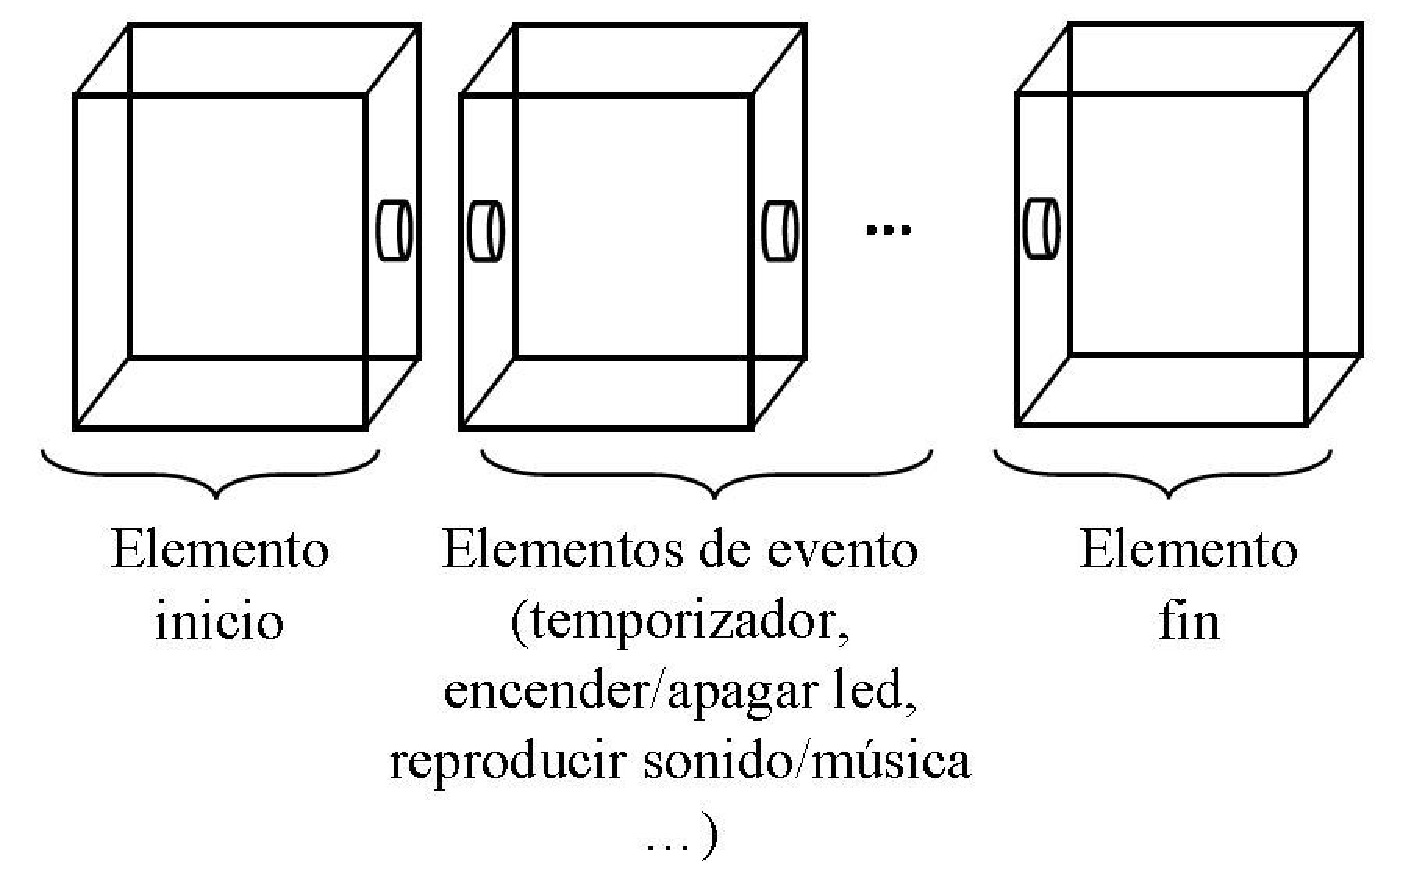
\includegraphics[width=0.7\textwidth]{Propuesta1cubos.pdf}
\caption{Diseño de la primera propuesta para el sistema tangible}
\label{fig:Propuesta1cubos}
\end{center}
\end{figure}

La comunicación con los diferentes cubos se realiza mediante bus serie de 4 líneas (entrada de datos, salida de datos, habilitación y señal de reloj).
Al ser ejecutado un programa, los diferentes cubos son iluminados de manera secuencial, es decir, desde el cubo elemento inicio, pasando por los diferentes cubos que realizan los eventos, hasta el cubo denominado fin.\
\textbf{Control de la iluminación de los cubos}.\
Cada uno de los cubos dispone de un número de identificación de 3 bits. El microcontrolador «ESP8266» establece una comunicación serie enviando una trama de 8 bits. Estos bits son almacenados en un registro de desplazamiento de entrada serie y salida en paralelo. Los bits más significativos son utilizados para identificar el cubo (3 bits, cubos del 0 al 7). Los bits menos significativos son utilizados para realizar la iluminación del cubo. La Figura~\ref{fig:Propuesta1registros}

\begin{figure}[!h]
\begin{center}
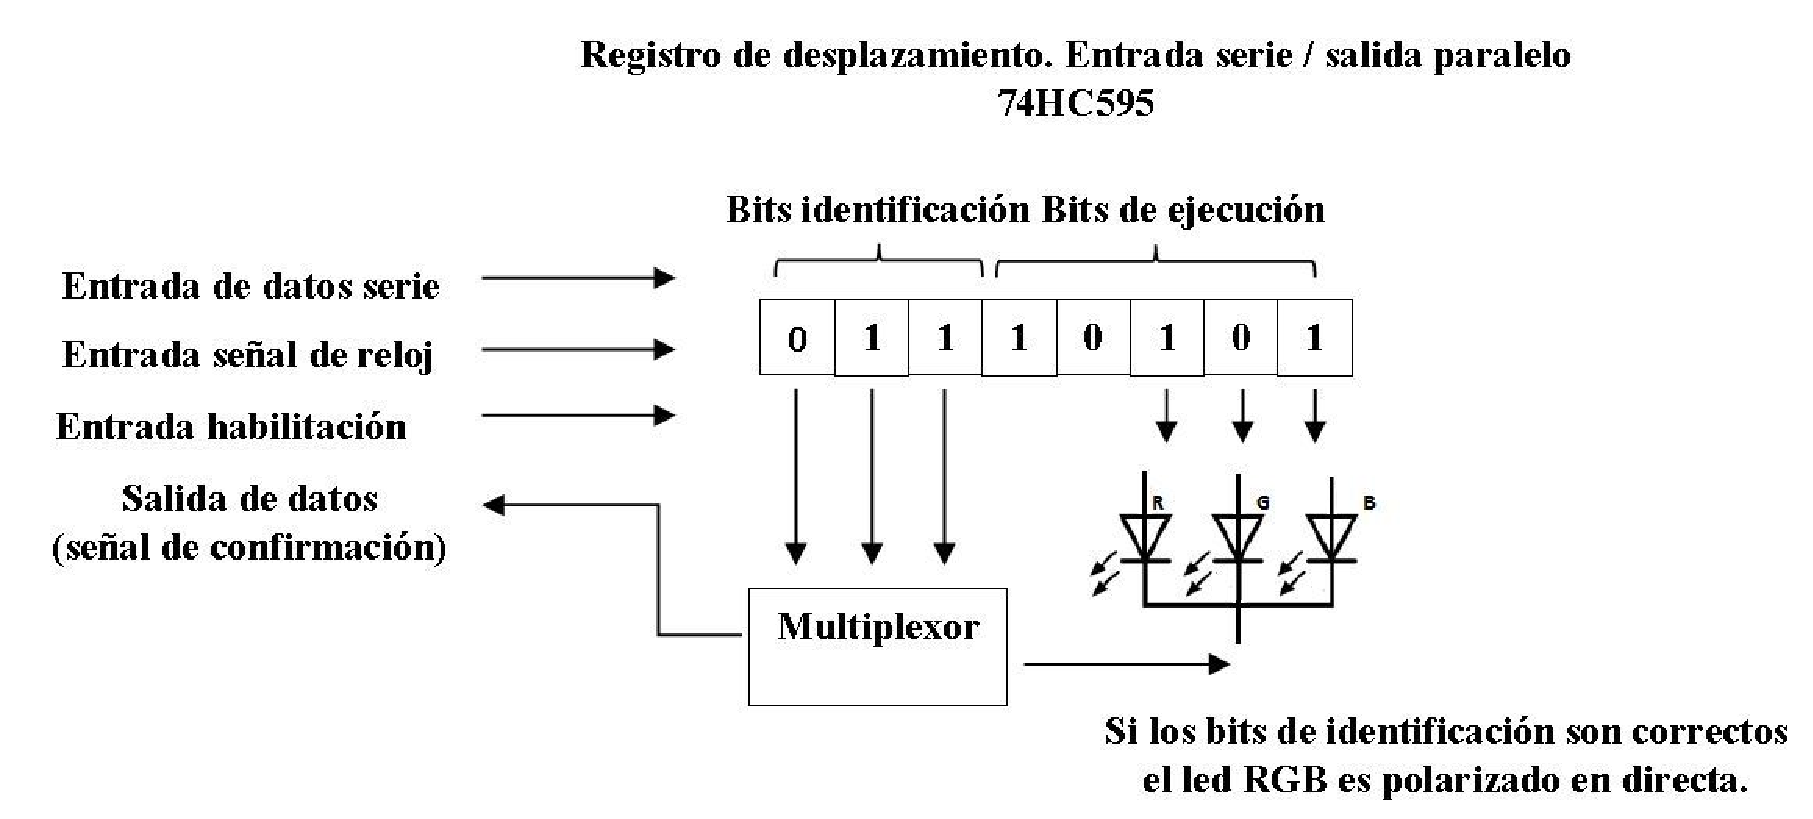
\includegraphics[width=0.7\textwidth]{Propuesta1registros.pdf}
\caption{Diseño de los registros de desplazamiento dentro de los cubos para indicar la posición de la secuencia dentro el sistema tangible}
\label{fig:Propuesta1registros}
\end{center}
\end{figure}

La comunicación entre los diferentes cubos se realiza mediante conectores magnéticos tipo «Micro USB». Al ser magnéticos facilita la conexión entre ellos.

\subsubsection{Resultados tras el análisis de la primera propuesta de diseño}

La primera propuesta de diseño queda descartada. Entre los motivos destaca el hecho de que actualmente en el mercado existen dispositivos de características muy similares, no aportando nada destacable, además de poder ser peligrosos los conectores magnéticos en una futura industrialización de la plataforma, al ser usado por niños.

Descartada la primera propuesta, se establece que el próximo objetivo es \textbf{ conocer el alcance del proyecto}, entendiendo que hay que construir, realizando un \textbf{estudio} más amplio que el realizado hasta ahora sobre los actuales sistemas tangibles enfocados a la programación tangible para niños. Además se ha de investigar sobre la \textbf{tecnología y características} que utilizan cada uno de ellos, para poder identificar cuáles son los puntos que se pueden mejorar en esos sistemas, y contribuir a mejóralos diseñando una plataforma de juego que resuelva todos esos puntos. Este análisis permitirá \textbf{establecer los requisitos} que debe tener la plataforma a diseñar, y que \textbf{tecnologías} utilizar en ella, para posteriormente establecer los pasos a realizar para alcanzar una serie de objetivos específicos dentro de la aplicación.\

\subsubsection{Próximas iteraciones e historias de usuario.}
Se acuerda para la próxima iteración los siguientes puntos:
\begin{itemize}
\item Estudio avanzado del problema. Revisión sistemática (recopilación de información).
\item Identificar áreas de mejora en los actuales sistemas tangibles.
\item Selección de las áreas de mejora para obtener los objetivos.
\end{itemize}


\subsection{Iteración 2: Estudio avanzado del problema. Identificación y selección de las áreas de mejora en sistemas tangibles.}

\subsubsection{Estudio avanzado del problema.}
En el \textbf{Capítulo Antecedentes} de este documento, se muestran los resultados sobre los principales estudios experimentales aplicados a la interacción tangible, y como motiva a niños de tempranas edades en sus habilidades computacionales. En ese capítulo se indican algunos de los dispositivos más importantes y que diferentes enfoques aportan en la interacción tangible, y que han sido utilizados para el aprendizaje computacional, así como sus características y tecnología utilizada. 
Realizado el análisis de los diferentes dispositivos, se exponen las áreas en los actuales sistemas tangibles.

\subsubsection{Áreas de mejora en sistemas tangibles.}
Los diferentes sistemas de interacción tangible tienen como propósito general que la
información sea comprensible y literalmente captable, haciendo uso de objetos físicos
que sean manipulables de una forma natural.\\
Otra de las características de la aplicación de los sistemas tangibles en el ámbito
educativo, es el entorno visual, que debe de motivar fuertemente al usuario, disponiendo
de un entorno de fácil uso e intuitivo, y que además fomente la capacidad de
razonamiento, creación e imaginación de los niños.\\
La evolución de la tecnología aplicada a los modelos actuales de sistemas tangibles, van
adaptándose para mejorar los diseños y conseguir de esta forma sistemas más fiables.
No obstante, existen diferentes áreas de mejora localizadas sobre los diferentes
sistemas de interacción tangible:\
\begin{itemize}
\item \textbf{Uso de elementos externos para su funcionamiento}. En algunos juegos es
imprescindible es uso de un ordenador para su normal funcionamiento (como es
el caso de Scratch \& WeDo), además del uso de periféricos, por ejemplo, el uso
de una cámara para el reconocimiento de imágenes.
\item \textbf{Elevado número de elementos tangibles para el desarrollo del juego}. Si bien es cierto que uno de los puntos más importantes a la hora de la programación para
niños, es poder representar partes de código de diferentes elementos tangibles,
un gran número de elementos puede suponer un problema para el niño a la hora
del desarrollo del juego, pudiendo en algunos casos confundirlo.
\item \textbf{Enfoque exclusivo de un rango de edades para el juego}. En la mayoría de los casos, los juegos están enfocados a niños de un determinado rango de edades,
limitando de esta manera el juego, ya que puede resultar de una dificultad
elevada para niños de corta edad, o demasiado fáciles para el resto de edades.
\item \textbf{Diseño estático del juego}. Una de las limitaciones de todos los juegos que hacen uso de interfaces tangibles, es que no pueden ser actualizados, o no disponen de
actualizaciones de software, lo que hace que el juego no evolucione e imposibilita posibles futuras mejoras en los juegos.
\item \textbf{Alto coste de los bloques o dispositivos de realimentación}. El uso de un gran número de elementos utilizados para la interacción tangible eleva el precio del
diseño.
\end{itemize}

\subsubsection{Próximas iteraciones e historias de usuario.}
Se acuerda para la próxima iteración los siguientes puntos:
\begin{itemize}
\item Establecer requisitos iniciales.
\item Identificar y redactar objetivos.
\item Investigación sobre las tecnologías a utilizar.
\item Historia de usuario: preparar una segunda propuesta de diseño según las áreas de mejora identificadas.
\end{itemize}


\subsection{Iteración 3: Establecer Requisitos Iniciales e Investigación sobre las Tecnologías a Utilizar}

Las áreas de mejora obtenidas en la Iteración 2 servirán de base para realizar la plataforma de juego. Se analiza cada punto para obtener la mejor solución posible, y que tecnología utilizar para cada caso.

\subsubsection{Uso de elementos externos al dispositivo}
El uso de elementos externos para el funcionamiento del juego, como por ejemplo el uso de un teclado o una pantalla que el propio usuario debe de disponer, en ocasiones puede acarrear un problema a la hora de utilizar el juego.\\ 
Para eliminar el uso de elementos externos para el funcionamiento del sistema de juego, se ha de conseguir diseñar un prototipo el cual precisa de dichos elementos, integrando todo lo necesario dentro de la misma plataforma. 

\subsubsection{Elevado número de piezas para la interacción tangible}
Un sistema de interacción tangible se caracteriza principalmente en que la información sea comprensible y literalmente captable, haciendo uso de objetos físicos que sean manipulables de forma natural. En ocasiones, el número de objetos físicos para el desarrollo del juego es elevado. Si bien es cierto que uno de los puntos más importantes a la hora de la programación para niños, es poder representar partes de código en diferentes elementos tangibles, un gran número de elementos puede suponer un problema para el niño a la hora del desarrollo del juego, pudiendo en algunos casos confundirlo. 

Los sistemas de programación tangible utilizan bloques que al conectarlos o posicionados de una manera concreta, generan en tiempo real movimientos o acciones, bien mostrando la acción realizada en una pantalla, o bien mediante algún tipo de robot articulado, etc... Cada bloque indica una acción, por ejemplo, bloque de inicio, bloque de fin, bloque de dirección, bloque sensor... 

Para dar solución a este problema, la idea pasa por intentar agrupar los bloques tangibles que son utilizados en los actuales juegos y que tienen como finalidad representar una acción, en un solo elemento tangible.

Se propone el diseño de un dispositivo tangible, que, por medio de un microprocesador, muestre en una pantalla estas funciones. 


\subsubsection{Enfoque exclusivo del juego en un rango de edades y diseño estático del juego}

La mayoría de los diseños actuales están enfocados a un rango de edades para el juego, ya que un determinado tipo de juego puede resultar demasiado simple o demasiado complejo para algunos niños debido a la edad de los mismos. 

Otro punto a tener en consideración es el diseño estático en los juegos de interacción tangible. El usuario dispone de unos recursos para ser utilizados, y aunque las combinaciones y posiciones de elementos tangibles permitan realizar diferentes acciones de juego, no dejan de ser siempre los mismos elementos con los mismos propósitos.

Estos dos puntos están relacionados con una característica común, y es que no tienen la posibilidad de mejorar, no pueden ser actualizados al menos que se compre una nueva versión del producto, lo perjudica al usuario final.

\textbf{Alto coste de los bloques o dispositivos de realimentación}
El alto coste de los bloques o dispositivos de realimentación al igual que el uso de un gran número de elementos utilizados para la interacción tangible, eleva el precio del
diseño.


Por lo tanto, los requisitos a implementar en la plataforma de juego son:
\begin{itemize}
\item \textbf{Dispositivo completo e independiente de elementos externos al mismo.}
\item \textbf{Agrupar los elementos tangibles que realizan las funciones en un solo dispositivo tangible.}
\item \textbf{Disponer de actualizaciones software para posibles mejoras en los juegos.}
\item \textbf{Utilización de elementos de bajo coste para el diseño }

\end{itemize}


Se procede a exponer y analizar la segunda propuesta de diseño de juego, basada en los requisitos expuestos.

\subsubsection{Historia de usuario: Segunda propuesta de diseño}

El sistema consta de dos cubos. Uno de mayor tamaño (cubo principal), que sirve de interfaz gráfica para la realización de los juegos, y otro cubo de menor tamaño (cubo auxiliar), utilizado de apoyo para la interacción del juego. De manera muy genérica se procede a la descripción de su estructura.\
\textbf{Descripción del cubo principal.}\

Dispone de una pantalla táctil para visualizar e interactuar con el juego. La estructura del cubo alberga el sistema de control («Raspberry Pi») y un conjunto de sensores. Los sensores que componen el cubo son los siguientes:
\begin{itemize}
\item \textbf{Sensores de proximidad:} situados en las cuatro caras que rodean la pantalla.
\item \textbf{Magnetómetro:} utilizado para detectar el cubo auxiliar en una posición concreta encima de la pantalla o en las proximidades del cubo principal.
\end{itemize}. La Figura~\ref{fig:Propuesta2cuboprincipal} muestra el diseño del cubo principal.\

\begin{figure}[!h]
\begin{center}
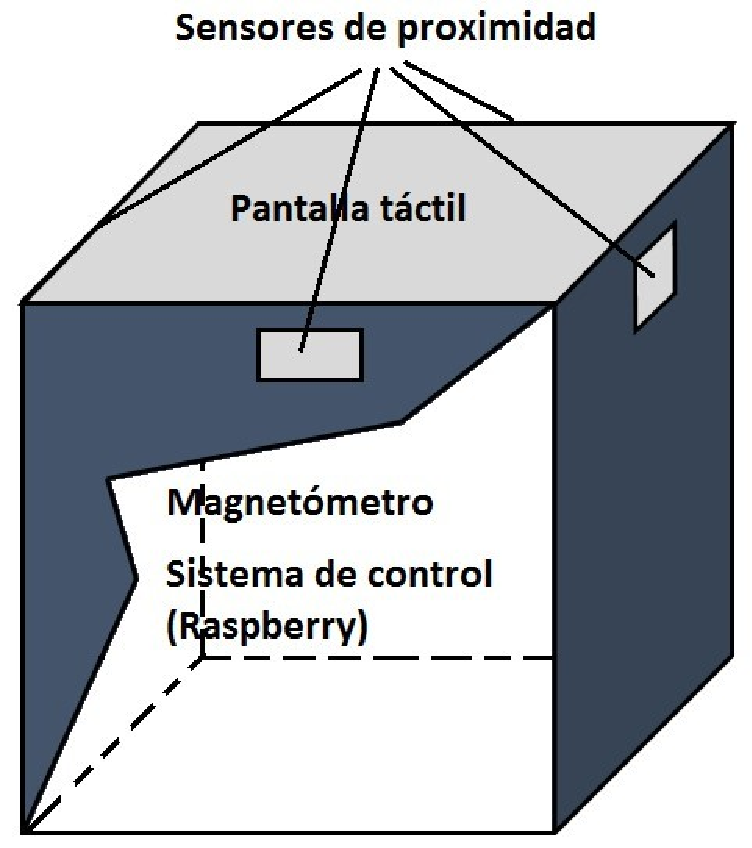
\includegraphics[width=0.3\textwidth]{Propuesta2cuboprincipal.pdf}
\caption{Diseño del cubo principal en la segunda propuesta de diseño}
\label{fig:Propuesta2cuboprincipal}
\end{center}
\end{figure}

\textbf{Descripción del cubo auxiliar.}\
El tamaño de este cubo es mucho menor que el principal para poder desplazarse por la pantalla del cubo principal. Dispone de una pantalla táctil en la parte superior.
Se hace uso de un giroscopio para determinar su orientación.
La propuesta para controlar los eventos generados y comunicarse con el cubo principal es el microcontrolador «ESP8266 ESP-12». Figura~\ref{fig:Propuesta2cuboaux}\

\begin{figure}[!h]
\begin{center}
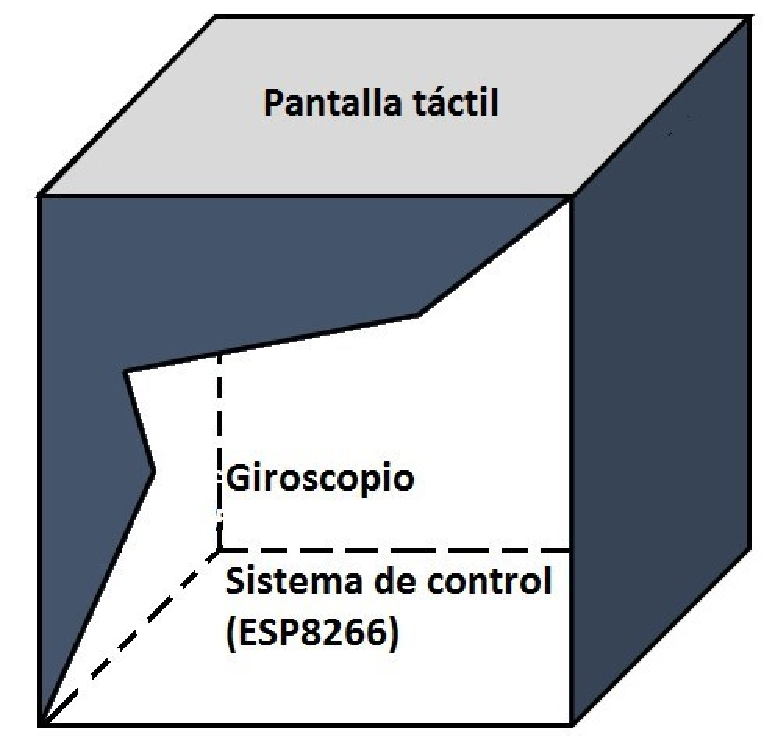
\includegraphics[width=0.3\textwidth]{Propuesta2cuboaux.pdf}
\caption{Diseño del cubo auxiliar en la segunda propuesta de diseño}
\label{fig:Propuesta2cuboaux}
\end{center}
\end{figure}


\textbf{Ejemplos de aplicaciones.}\
Se proponen algunas propuestas de juegos de manera muy básica, donde son utilizados los diferentes sensores de la plataforma de juego. Se hace uso de colores por simplicidad en la explicación.

\begin{itemize}
\item \textbf{Definir una secuencia.} La pantalla del cubo principal se divide en nueve secciones para que la interacción sea más intuitiva.
A continuación, se define el recorrido que tendrá el juego deslizando el dedo sobre la
superficie de la pantalla (por ejemplo como se muestra en la Figura~\ref{fig:Propuesta2secuencia1}).
\begin{figure}[!h]
\begin{center}
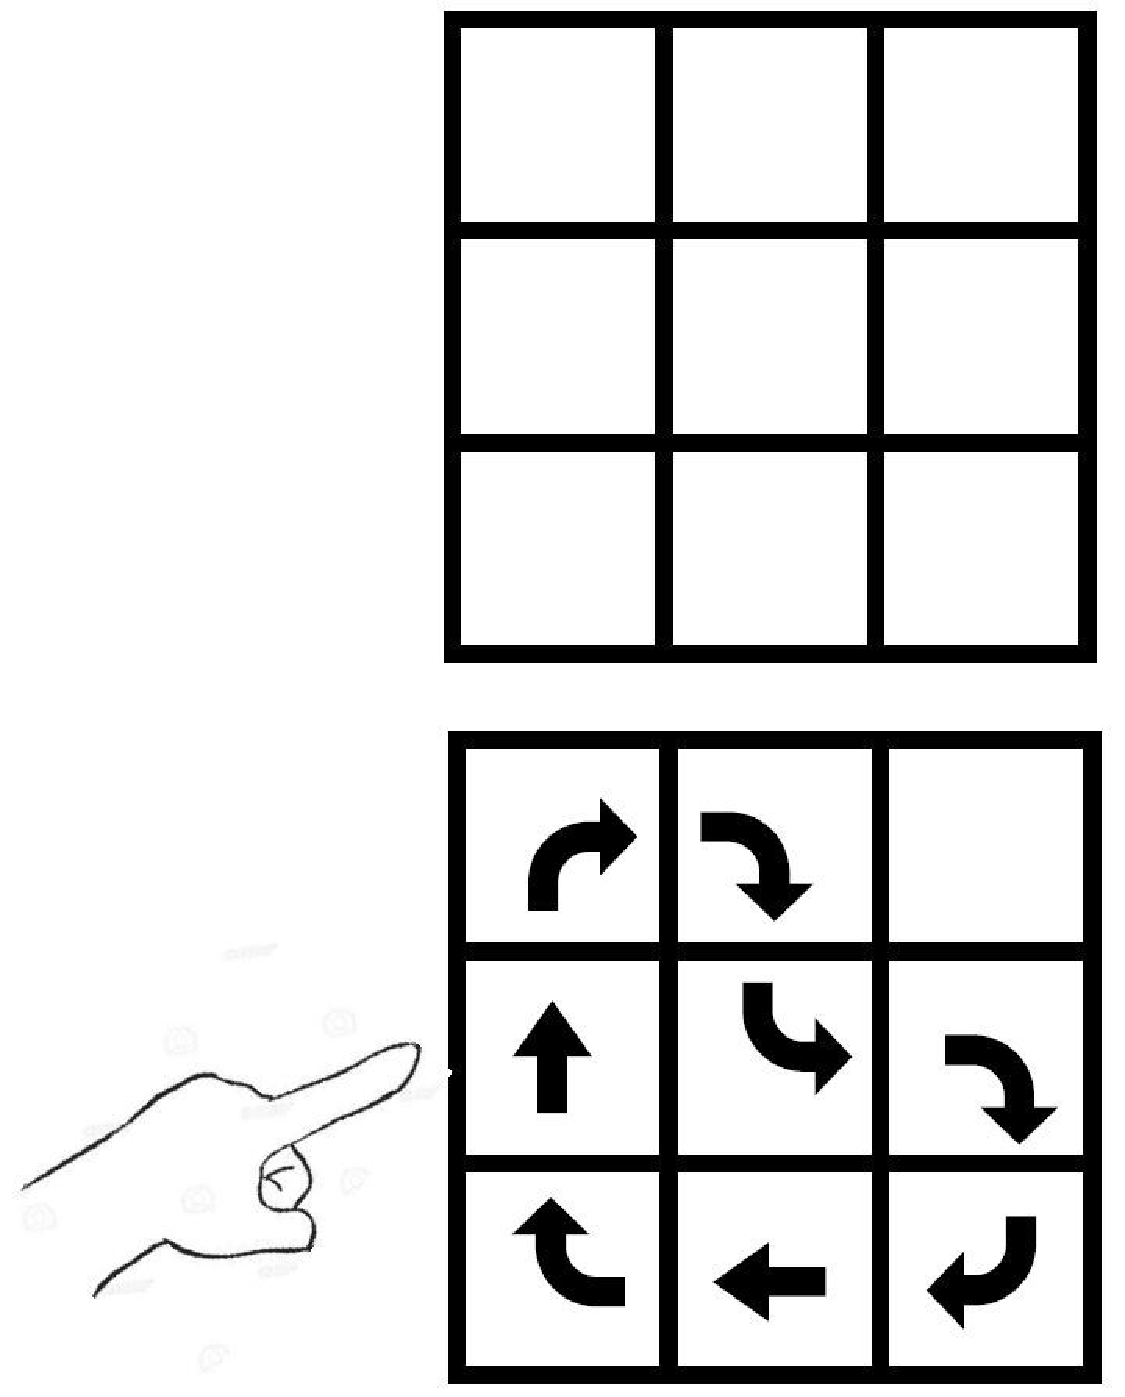
\includegraphics[width=0.3\textwidth]{Propuesta2secuencia1.pdf}
\caption{Definir una secuencia en el cubo principal de la segunda propuesta de diseño}
\label{fig:Propuesta2secuencia1}
\end{center}
\end{figure}
El programa comienza a ejecutarse en función del recorrido marcado, desplazándose de un cuadro a otro. Como ejemplo simple se hace uso de un cuadrado de color verde que se desplaza sobre el tablero (ver Figura~\ref{fig:Propuesta2secuencia2}).\

\begin{figure}[!h]
\begin{center}
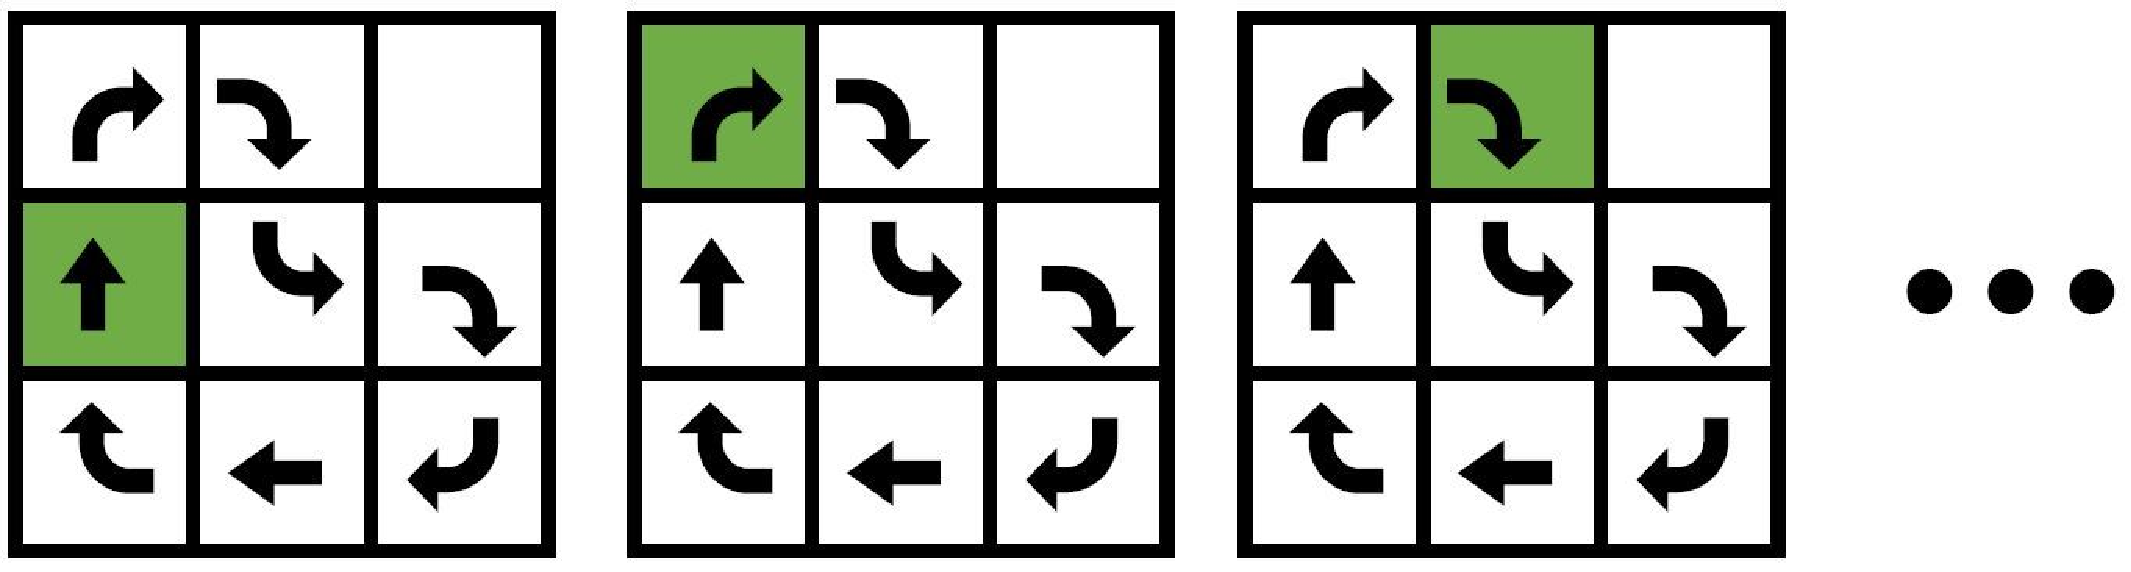
\includegraphics[width=0.4\textwidth]{Propuesta2secuencia2.pdf}
\caption{Desarrollo de la secuencia en el cubo principal de la segunda propuesta de diseño}
\label{fig:Propuesta2secuencia2}
\end{center}
\end{figure}

\item \textbf{Uso de sensores de proximidad.} Acercando la mano en las proximidades de los laterales donde se encuentran estos sensores el cuadro es desplazado siendo la secuencia alterada (ver Figura~\ref{fig:Propuesta2secuencia3}).\

\begin{figure}[!h]
\begin{center}
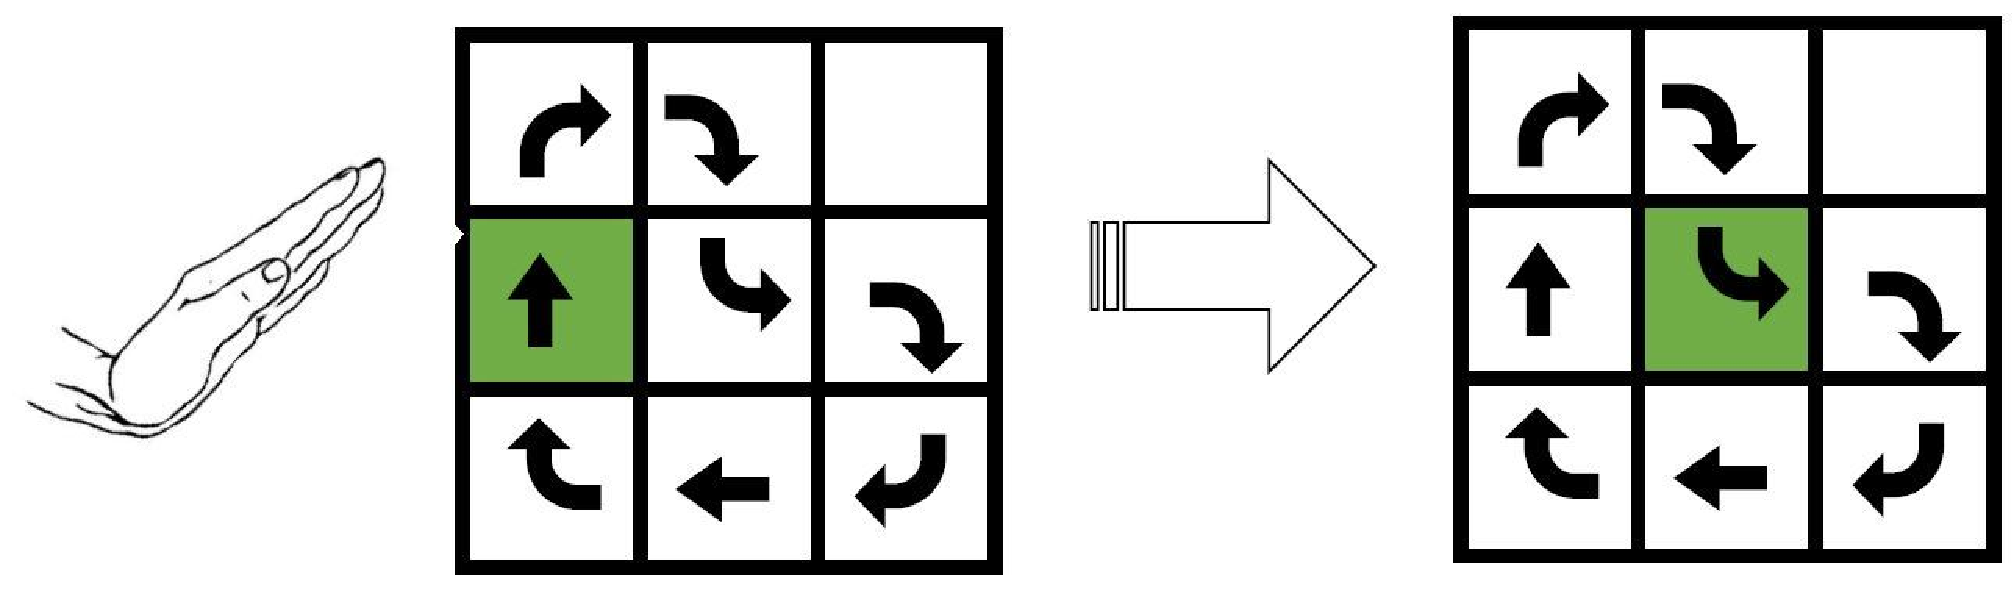
\includegraphics[width=0.4\textwidth]{Propuesta2secuencia3.pdf}
\caption{Modificación de la secuencia en el cubo principal mediante el uso de sensores de proximidad en la segunda propuesta de diseño}
\label{fig:Propuesta2secuencia3}
\end{center}
\end{figure}


\item \textbf{Interacción entre ambos cubos.} Se pretende realizar una interacción directa entre los dos cubos, dando lugar a un intercambio de información entre ambos elementos, permitiendo modificar la secuencia realizada directamente con el cubo auxiliar. Como ejemplo se propone realizar una «captura» dentro de la secuencia. La idea es posicionar el cubo auxiliar sobre el cubo principal para realizar una «captura» sobre el cuadro activo, eliminando de la secuencia este cuadro (ver Figura~\ref{fig:Propuesta2secuencia4}). Una vez «capturado» el cuadro, se puede modificar los atributos del mismo tocando sobre la pantalla del cubo auxiliar (ver Figura~\ref{fig:Propuesta2secuencia5}).

\begin{figure}[!h]
\begin{center}
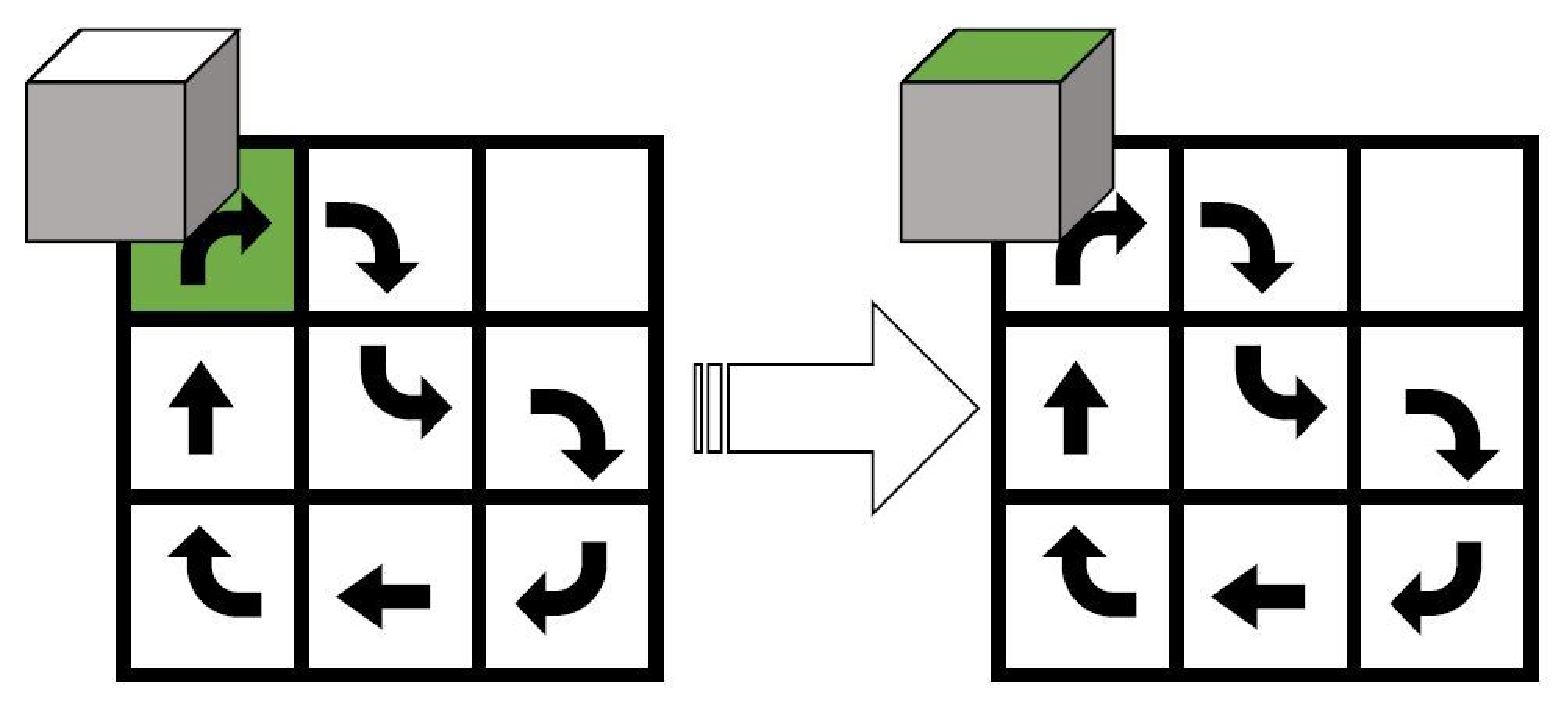
\includegraphics[width=0.4\textwidth]{Propuesta2secuencia4.pdf}
\caption{Captura del cuadro activo dentro de la secuencia en el cubo principal, mediante el uso del cubo auxiliar en la segunda propuesta de diseño}
\label{fig:Propuesta2secuencia4}
\end{center}
\end{figure}

\begin{figure}[!h]
\begin{center}
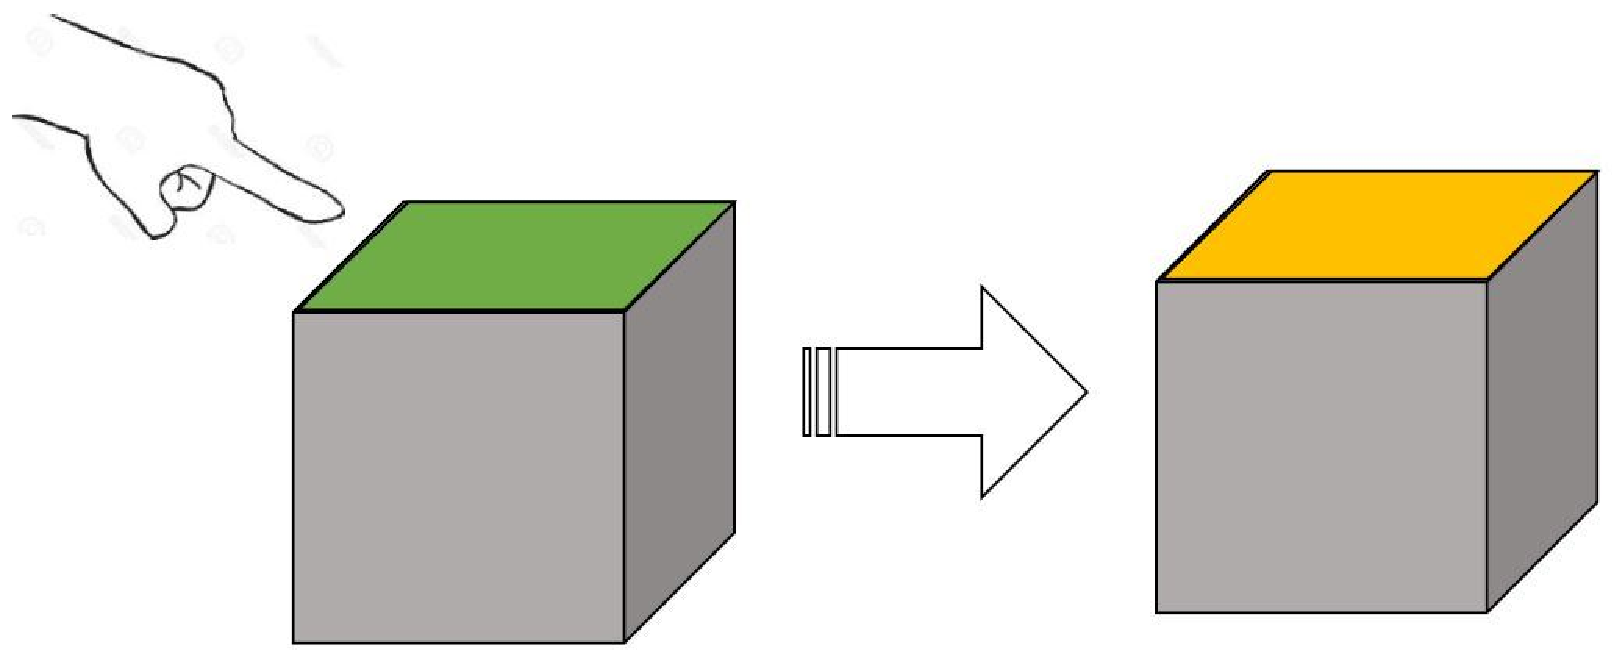
\includegraphics[width=0.4\textwidth]{Propuesta2secuencia5.pdf}
\caption{Modificación de la secuencia en el cubo principal mediante el uso del cubo auxiliar en la segunda propuesta de diseño}
\label{fig:Propuesta2secuencia5}
\end{center}
\end{figure}

Posteriormente se emplaza en otra localización para continuar la secuencia (Figura~\ref{fig:Propuesta2secuencia6}).

\begin{figure}[!h]
\begin{center}
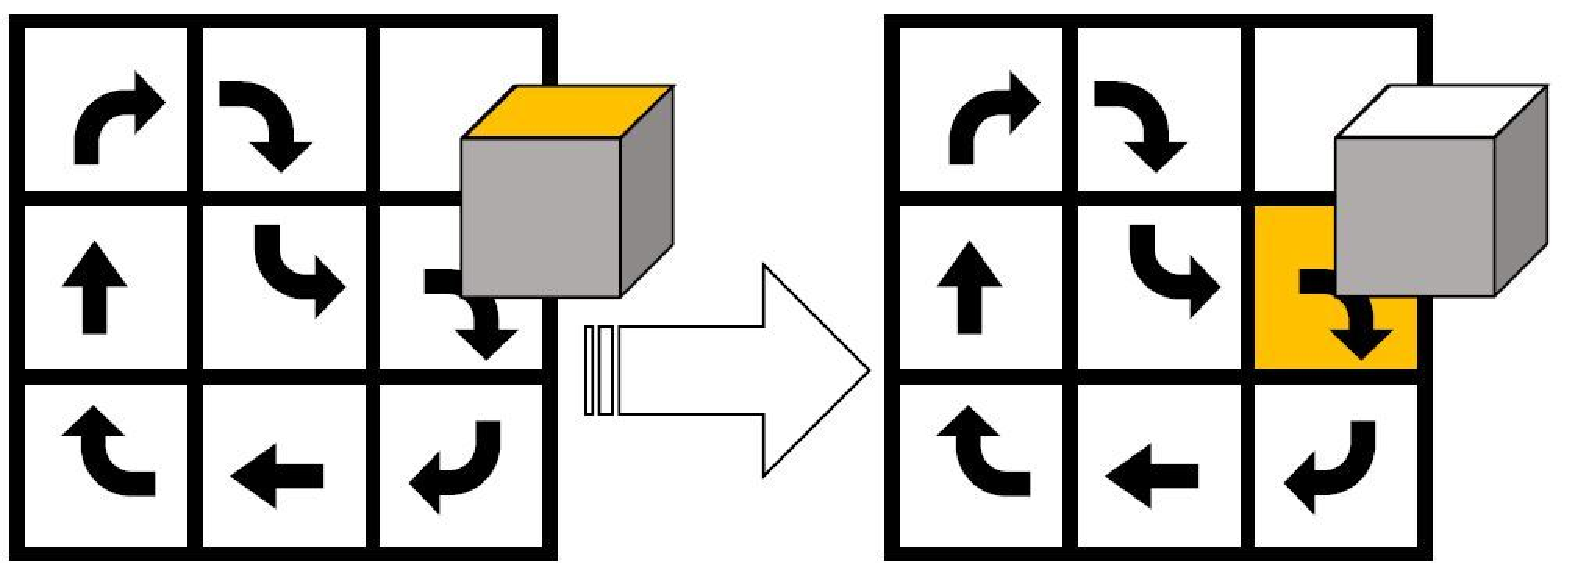
\includegraphics[width=0.4\textwidth]{Propuesta2secuencia6.pdf}
\caption{Emplazamiento dentro de la secuencia en el cubo principal del cuadro modificado, mediante el uso del cubo auxiliar en la segunda propuesta de diseño}
\label{fig:Propuesta2secuencia6}
\end{center}
\end{figure}

\end{itemize}


\subsubsection{Resultados tras el análisis de la segunda propuesta de diseño}
Junto con \textbf{Francisco Moya Fernández} se decide aceptar la segunda propuesta de diseño ya que cumple con los requisitos establecidos. Se acuerda realizar algunas modificaciones al encontrar posibles futuros problemas en ciertos puntos del diseño. Estos posibles problemas son:
\begin{itemize}
\item \textbf{Localización del dispositivo de menor tamaño sobre el de mayor tamaño, mediante un magnetómetro.} Debido a que el sensor no ofrecerá la precisión necesaria que requiere la aplicación para indicar una localización exacta del dispositivo respecto a otro, se decide eliminar esta característica a la espera de \textbf{buscar una solución} para la localización, quedando pendiente como próxima historia de usuario en la siguiente iteración.
\item \textbf{Tamaño de las pantallas de ambos dispositivos y microcontrolador del dispositivo de menor tamaño.} La opción de utilizar el microcontrolador «ESP8266» queda descartada debido a posibles problemas en el flujo de datos en el transcurso del juego, ya que posiblemente, la visualización del entorno gráfico no sea adecuada. Por otro lado, el tamaño de las pantallas no está definido, quedando como próxima historia de usuario al igual que establecer un nuevo sistema de procesamiento de datos.
\end{itemize}

Las características y elementos aceptados en la propuesta de diseño son:\
\begin{itemize}
\item \textbf{Desarrollar la plataforma de juego con dos dispositivos (uno de mayor tamaño que el otro).}
\item \textbf{Sistema de visualización mediante pantalla en ambos dispositivos.}
\item \textbf{«Raspberry Pi» como elemento principal de procesamiento de datos en el dispositivo de mayor tamaño.}
\item \textbf{Implementación de sensores ópticos e inerciales.} 
\item \textbf{Uso de la interacción directa entre ambos dispositivos, para la localización del elemento de menor tamaño sobre el de mayor tamaño.}
\end{itemize}

Todas estas características cumplen con los requisitos iniciales del sistema, y serán aplicadas en el diseño final de la plataforma de juego, quedando abierta la posibilidad de añadir futuras modificaciones sobre las ya implementadas.

\subsubsection{Próximas iteraciones e historias de usuario.}
Se acuerda para la próxima iteración los siguientes puntos:
\begin{itemize}
\item Establecer objetivos específicos.
\item Finalizar estudio tecnológico para establecer tecnologías a utilizar.
\item Historia de usuario: sistema de localización entre ambos dispositivos.
\item Historia de usuario: procesamiento de datos del dispositivo de menor tamaño, y establecer tamaños en pantallas de ambos dispositivos
\end{itemize}


\subsection{Iteración 4: Establecer Objetivos y Tecnologías a Utilizar}

En esta iteración se define el objetivo general del presente Trabajo Fin de Grado, así como los objetivos específicos que definirán el transcurso del resto de iteraciones hasta obtener el resultado deseado, quedando abierta la posibilidad de modificar dichos objetivos específicos acorde con las necesidades del dispositivo.

\subsubsection{Objetivos del TFG}


\textbf{Objetivo general}: Diseñar y desarrollar una plataforma interactiva de juego de bajo coste, basada en interfaces tangibles, haciendo uso de las nuevas tecnologías, para promover el desarrollo de capacidades en niños de corta edad.

\textbf{Objetivos específicos}:
\begin{itemize}
\item Diseñar y programar un sistema de localización y reconocimiento de las interfaces de usuario tangibles.

\item Desarrollar un sistema eficiente de transferencia de datos entre ambas interfaces tangibles.

\item Realizar una correcta sincronización en la visualización de la aplicación entre ambas pantallas, que permita una buena representación de juego.

\item Ofrecer un entorno gráfico simple, que permita al niño ser capaz de diseñar secuencias y modificarlas interactuando con los elementos tangibles.

\item Adaptar sensores inerciales y ópticos para una mejor experiencia de juego, donde ambos elementos tangibles interactúen entre sí, permitiendo la manipulación de la información entre los dispositivos.

\item Diseñar un sistema de actualización de software de los dispositivos, a través de la conexión externa a un servidor.
\end{itemize}

\subsubsection{Historia de usuario: Sistema de localización entre ambos dispositivos}
De manera conjunta con las búsquedas de nuevas tecnologías, y antes de proceder a exponer que tecnologías utilizar, se formula la propuesta del sistema de localización entre dispositivos, para ser valorada junto con \textbf{Francisco Moya Fernández}.

El sistema de localización que se plantea para dar solución a la poca precisión de un magnetómetro en este tipo de aplicaciones, es hacer uso de una pantalla multitáctil capacitiva en el dispositivo de mayor tamaño. El dispositivo de menor tamaño a su vez, dispone de unas almohadillas conductivas en su parte inferior, de forma que al ser posicionado sobre la superficie de la pantalla capacitiva, ésta detecte el contacto de las almohadillas, indicando las coordenadas de posición del dispositivo de menor tamaño. 

Para realizar el sistema de localización se identifican los dos dispositivos principales mediante acrónimos. El elemento de mayor tamaño es denominado como «TUIO1». A su vez se define el dispositivo de menor tamaño como «TUIO2». El motivo de elegir estos nombres, es por el hecho de que «TUIO» son las siglas en ingles de \textbf{Tangible User Interface Object}.

Lo que se pretende obtener es una interacción directa entre dispositivos, ofreciendo la posibilidad de intercambiar información durante el desarrollo de un juego, tal y como se expuso en la \textbf{Iteración 3}, en los ejemplos de juegos en la segunda propuesta de diseño.

Uno de los requisitos iniciales expuestos en la \textbf{Iteración 3}, es reducir el número de piezas utilizadas, agrupando los bloques tangibles y que tienen como finalidad representar una acción durante el transcurso de la creación de una secuencia en el juego, en un solo elemento tangible, que sea capaz de representar ese tipo de eventos. El elemento de menor tamaño «TUIO2», es el encargado de este cometido, actuando como «Widget tangible», que situado sobre la pantalla táctil capacitiva del dispositivo «TUIO1» representa de manera gráfica estas acciones.

La propuesta de hacer uso de una pantalla multitáctil capacitiva para el sistema de localización es aceptada, y será incluida en las tecnologías utilizadas expuestas en esta interacción.

\subsubsection{Historia de usuario: Procesamiento de datos del dispositivo de menor tamaño, y establecer tamaños en pantallas de ambos dispositivos }

Para corregir los posibles problemas que puede causar en el entorno gráfico en el dispositivo de menor tamaño al utilizar el microcontrolador «ESP8266» a la hora de ejecutar la aplicación, se plantea el uso de «Raspberry Pi», al igual que en el dispositivo de mayor tamaño.\

Dado que la plataforma de juego está orientada a niños de corta edad, el tamaño de las pantallas debe ser el adecuado para una correcta visualización de los juegos. Se sugiere el uso de un tamaño de 7 pulgadas para el dispositivo de mayor tamaño «TUIO1», y otro de 3,5 pulgadas para el dispositivo de menor tamaño «TUIO2».

Tras evaluar ambas propuestas conjuntamente con \textbf{Francisco Moya Fernández}, son aceptadas y serán añadidas a la lista de tecnologías a utilizar.


\subsubsection{Tecnologías a utilizar.}

Abordado el \textbf{estudio del problema}, efectuada la \textbf{recopilación de información} sobre los actuales juegos de programación tangible para niños, realizando un \textbf{análisis del problema}, efectuada la \textbf{investigación de las tecnologías} e \textbf{identificando las áreas de mejora} para marcar unos \textbf{requisitos iniciales} que permitan definir unos \textbf{objetivos} para la plataforma de juego, se procede a exponer las tecnologías que van a ser implementadas.\ 

Los elementos tecnológicos que serán integrados en la plataforma de juego, son elegidos acorde con las propuestas de diseño, de las cuales se extrajeron aquellos elementos que cumplían con los requisitos iniciales. Esta lista de componentes es una \textbf{lista abierta}, y podrá ser modificada durante el transcurso del sistema, de acuerdo a las necesidades del mismo:

\begin{itemize}
\item \textbf{Placa para el desarrollo.} Todos los eventos generados en la plataforma de juego para ambos dispositivos serán manejados mediante el computador de placa única \textbf{«Raspberry Pi 3»}. Esta placa dispone de un microprocesador «BCM2837» de 64 bits de cuádruple núcleo a 1,2GHz, 1GB de memoria RAM y GPU de doble núcleo Videocore IV, que permite manejar y procesar eventos e imágenes según los requisitos de la aplicación.
Integra el chip «BCM43143» para la comunicación Wi-Fi entre dispositivos, lo que elimina la necesidad de utilizar cables. Para el uso de la interfaz gráfica de usuario mediante dispositivo de salida (pantalla LCD), dispone de un puerto de vídeo/audio HDMI. Incorpora 40 pines GPIO, los cuales disponen de un bus «I2C» \footnote{I2C, «Inter-Integrated Circuit».} para la utilización de sensores dentro del sistema de juego, y un bus «SPI»\footnote{SPI, «Serial Peripheral Interface» } como alternativa al puerto HDMI para mostrar la interfaz gráfica de usuario.
Su reducido tamaño, bajo consumo, además de contar con una gran comunidad de usuarios, hacen de este dispositivo el adecuado para la realización de un prototipo de plataforma de juego.
\item \textbf{Pantallas.} Para el dispositivo «TUIO1», es utilizada una pantalla LCD con un tamaño de 7 pulgadas. Este tamaño es adecuado para una correcta visualización de los contenidos del juego. La pantalla dispone de un panel multitáctil tipo capacitivo, que permitirá gestionar los eventos generados sobre el mismo. La conexión con la placa para el desarrollo para la visualización de la interfaz gráfica, se realiza mediante puerto HDMI.
Los eventos táctiles son administrados mediante conexión USB.\
El dispositivo «TUIO2» dispone de una pantalla LCD, de un tamaño de 3,5 pulgadas que utiliza un panel táctil resistivo para captar los eventos de entrada. Este tamaño permite visualizar los contenidos en el desarrollo del juego, de manera que ofrece una interacción con la interfaz gráfica adecuada. La conexión con la placa para el desarrollo es mediante comunicación «SPI».
\item \textbf{Sensores.} Los sensores integrados en la plataforma de juego son, un sensor inercial «MPU9250», y un sensor óptico. Ambos sensores dedicados a efectuar una interacción entre ambos dispositivos. El elemento «TUIO2» dispone de ambos sensores, y es el encargado de recibir los eventos generados, para posteriormente transmitir dichos eventos vía Wi-Fi con el dispositivo «TUIO1».\

\item \textbf{Sistema operativo y entorno de programación.} Para el desarrollo de la aplicación, se utilizará la distribución gratuita \textbf{«KivyPie»}. Esta distribución incluye el sistema operativo \textbf{«PipaOS»} basado en \textbf{«Raspbian»}, utilizado en proyectos hardware desde cero, que contiene el software mínimo para poner «Raspberry Pi» en funcionamiento. Incluye la herramienta para desarrollo \textbf{«Kivy».} Esta herramienta es un entorno de trabajo para aplicaciones multitáctiles de \textbf{«Python».}
\end{itemize}

Junto con \textbf{Francisco Moya Fernandez} se acuerda que las herramientas para el desarrollo de los programas de la plataforma de juego sean \textbf{Kivy} y \textbf{Python}. Se han elegido ambos lenguajes de programación debido a la facilidad y simplicidad de los mismos para desarrollar programas y entornos gráficos en aplicaciones con dispositivos multitáctiles.


Las características expuestas, y la descripción de dispositivos y entornos de programación, están reflejadas en el capitulo.

\subsubsection{Próximas iteraciones e historias de usuario.}
Se acuerda para la próxima iteración los siguientes puntos:
\begin{itemize}
\item Iniciar sistema de localización en pantalla táctil capacitiva.
\item Programa de pruebas para las comunicaciones entre dispositivos. 
\end{itemize}


\subsection{Iteración 5: Inicio del sistema de localización entre dispositivos y pruebas en las comunicaciones }

En esta iteración se tratan dos de los puntos más importantes de la plataforma de juego, como es \textbf{la localización del dispositivo «TUIO2», sobre «TUIO1»}, y como ambos elementos intercambian información mediante comunicación inalámbrica.

\subsubsection{Sistema de localización.}

El sistema de localización consiste en obtener las coordenadas de la posición del «Widget tangible TUIO2» sobre la pantalla táctil capacitiva del dispositivo «TUIO1», con el objetivo de generar un «efecto cristal», es decir, obtener una representación gráfica en la pantalla de «TUIO2», del cuadrante correspondiente a la representación gráfica de «TUIO1», y que cubre el dispositivo «TUIO2», como puede ser una imagen o una animación.\

Para entender mejor el sistema de localización se presenta el siguiente ejemplo. Antes de posicionar «TUIO2» sobre «TUIO1», las pantallas de ambos dispositivos muestran imágenes diferentes (ver Figura~\ref{fig:Localizacion1}).
\begin{figure}[!h]
\begin{center}
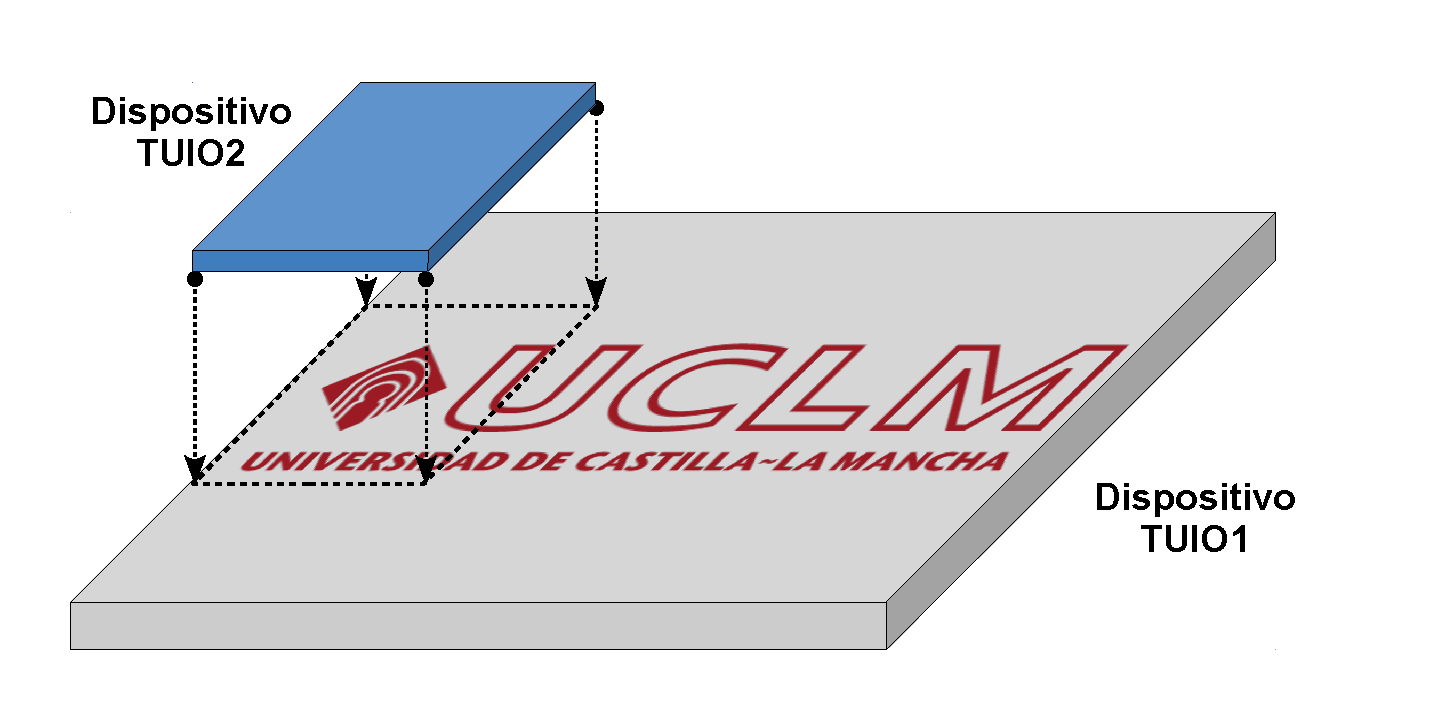
\includegraphics[width=0.7\textwidth]{localizacion1.pdf}
\caption{Posición de los dispositivos antes de la interacción sobre la pantalla capacitiva}
\label{fig:Localizacion1}
\end{center}
\end{figure}
Al posicionar «TUIO2» sobre la pantalla de «TUIO1», la pantalla de «TUIO2» muestra la parte de imagen correspondiente que es tapada por el dispositivo (Figura~\ref{fig:Localizacion2}).
\begin{figure}[!h]
\begin{center}
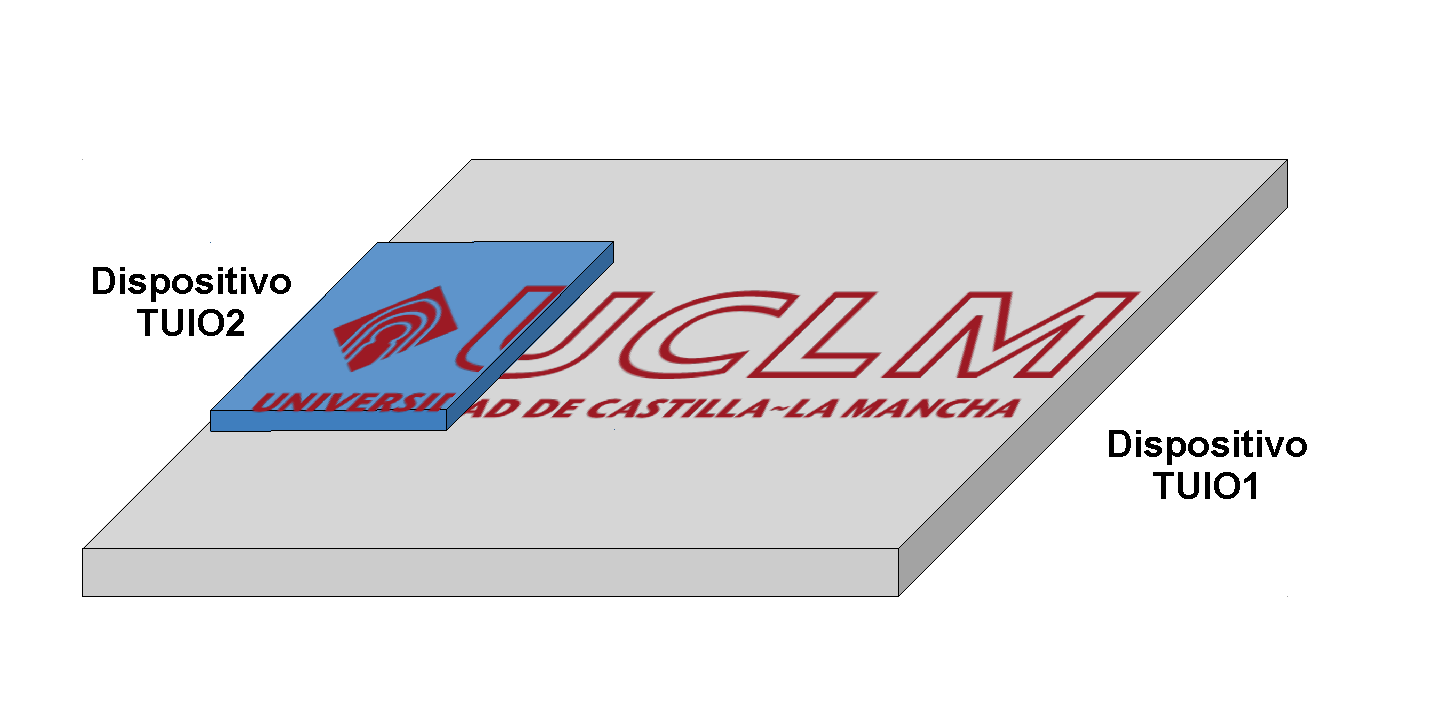
\includegraphics[width=0.7\textwidth]{localizacion2.pdf}
\caption{Posición de los dispositivos después de la interacción sobre la pantalla capacitiva}
\label{fig:Localizacion2}
\end{center}
\end{figure}

El procedimiento para obtener la posición, se consigue mediante el uso del sensor capacitivo de la propia pantalla de «TUIO1», que al detectar una variación de la capacitancia genera un evento táctil.
El dispositivo «TUIO2» produce tres eventos táctiles sobre la pantalla capacitiva. Estos eventos son generados por medio de tres almohadillas de goma conductora, que están conectadas al borne negativo de la «RaspberryPi». Esta conexión evita que el usuario tenga que sostener con su propia mano el dispositivo, haciendo de conexión a tierra el propio borne negativo.
El diseño de los puntos de contacto es el que se muestra en la Figura~\ref{fig:Localizacion3}.
\begin{figure}[!h]
\begin{center}
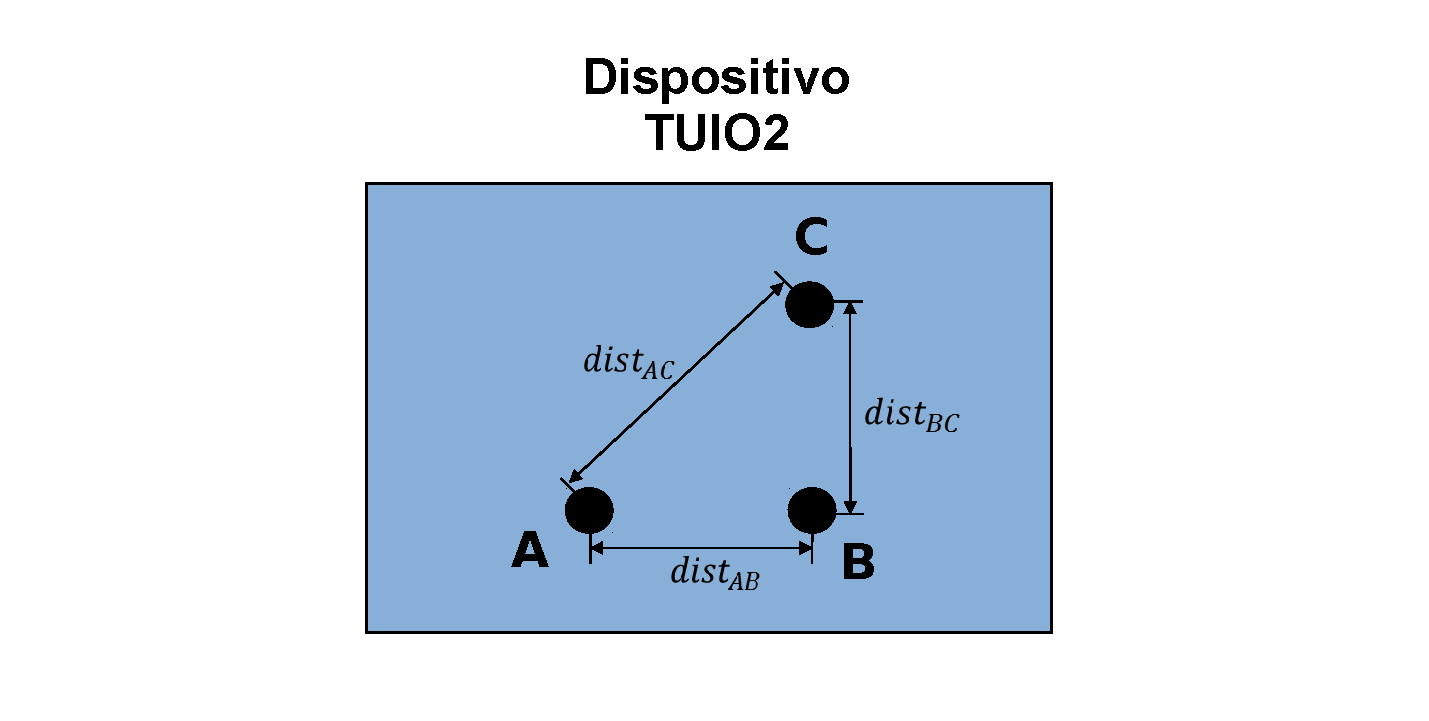
\includegraphics[width=0.9\textwidth]{localizacion3.pdf}
\caption{Disposición de las almohadillas conductoras en la parte inferior del «Widget tangible» para generar los eventos táctiles. }
\label{fig:Localizacion3}
\end{center}
\end{figure}
Los tres puntos de contacto son identificados A, B y C, que dan nombre a los vértices del triángulo rectángulo escaleno que forman. Se ha elegido este tipo de diseño ya que cada uno de los tres lados tiene una medida diferente, lo que hace que sea más fácil identificar cada segmento del triángulo, y así evitar posibles problemas cuando se localice cualquiera de sus vértices.

Cuando «TUIO2» está sobre la pantalla, los eventos táctiles generados, proporcionan la siguiente información al dispositivo «TUIO1»: posición e ID del evento. Las coordenadas de la posición de cada evento táctil está expresada en pixels, por lo que cada evento producido será manejado en esas unidades de media (ver Figura~\ref{fig:Localizacion4}).\\
\begin{figure}[!h]
\begin{center}
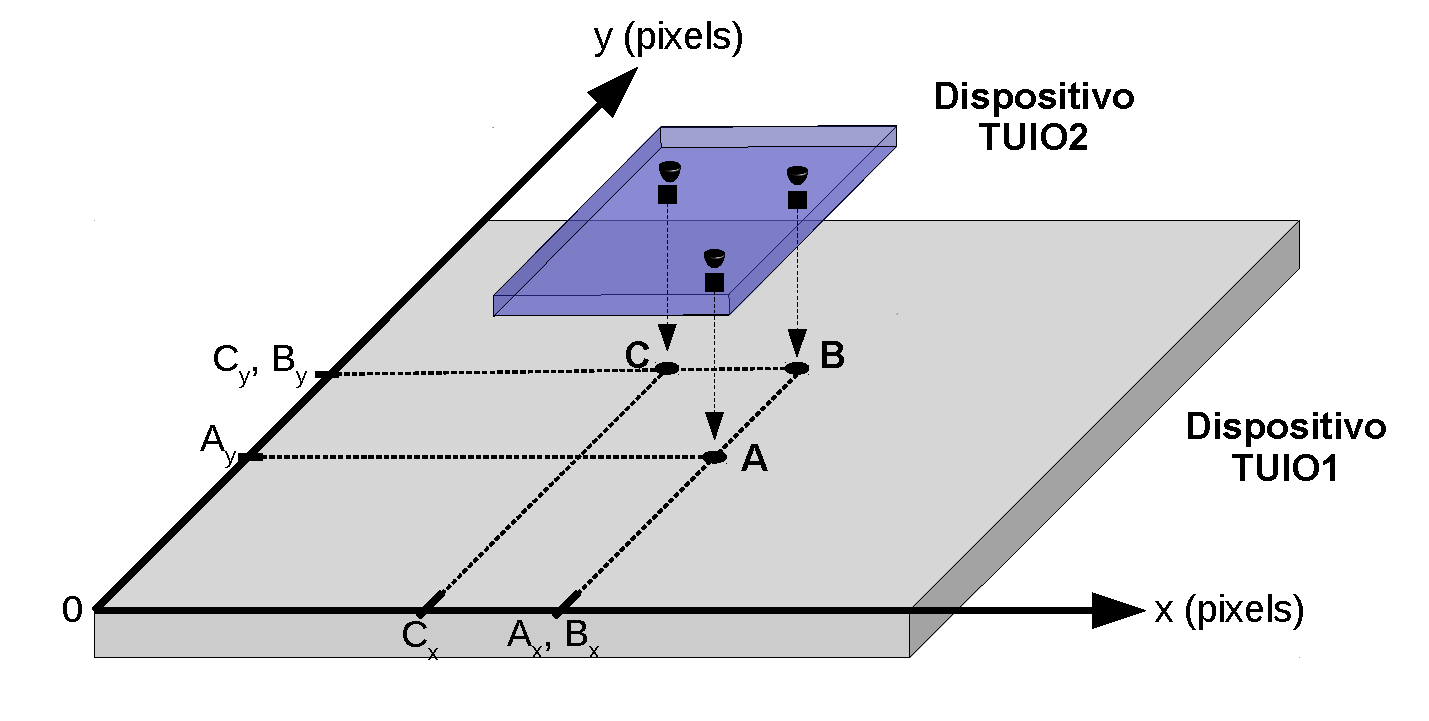
\includegraphics[width=0.9\textwidth]{localizacion4.pdf}
\caption{Coordenadas de los puntos A, B y C del «Widget tangible» sobre la pantalla capacitiva. }
\label{fig:Localizacion4}
\end{center}
\end{figure}
Estos datos son interpretados y tratados para calcular la posición de «TUIO2» mediante una librería que ha sido desarrollada en \textbf{Python} por el propio autor del TFG.

\subsubsection{Librería para la localización.}

Todos los eventos táctiles generados sobre la pantalla capacitiva del dispositivo «TUIO1» son manejados por la \textit{clase Widget} en \textbf{Python}, mediante el método \texttt{on\_touch\_down().}\\
Este método obtiene la información de posición e ID del evento táctil producido, almacenando estos datos en la lista \texttt{touch[].}\\
Se crea una librería específica para el manejo de esta lista, la cual tratará y manejara los datos para obtener la información de posición de «TUIO2».

\textbf{Método \texttt{pulsacion(touch)}}\\
El argumento de entrada corresponde con las coordenadas y la id del evento táctil que contiene la lista de eventos (\texttt{touch}).\\
Estos datos son almacenados en la última posición de la lista \texttt{puls[]} mediante el método \texttt{append()}:\\
\texttt{self.puls.append((t.x,t.y,t.id))}.\\
donde: \\
\texttt{t.x}: coordenada x del evento táctil.\\
\texttt{t.y}: coordenada y del evento táctil.\\
\texttt{t.id}: identificación del evento táctil (número de evento).\\
Cuando el número de eventos almacenados en \texttt{puls[]} 
es mayor que 1, se llama al método \texttt{determinar\_distancias()}.

\textbf{Método \texttt{determinar\_distancias()}}.\\
Mediante el método \texttt{Vector()}, de la librería \texttt{kivy}, es determinada la distancia entre los eventos táctiles producidos hasta el momento, y que son almacenados en la lista \texttt{puls[]}, haciendo uso de un bucle el cual recorre desde el último elemento de la lista \texttt{puls[]} hasta el primero. El método \texttt{determinar\_lados} es llamado en cada medida que se realiza de la distancia. Si la distancia es correcta, se incrementa la variable \texttt{contador}, la cual al llegar a 2, llama al método \texttt{determinar\_puntos()}.

\textbf{Método \texttt{determinar\_lados()}}.\\
Método para verificar si los dos eventos táctiles de los cuales se han determinado la distancia, corresponden con uno de los lados del triángulo del \textit{Widget tangible}, donde \textit{m} corresponde con la distancia entre los dos eventos táctiles, \textit{i} el tamaño de la lista \texttt{puls[]}, y \textit{a} el número de iteración del bucle que recorre cada uno de los elementos de la lista \texttt{puls[]}.

Este método es llamado cada vez que el método \texttt{determinar\_distancias()} es invocado.
Se comprueba si la distancia entre los dos puntos corresponde con el rango de medidas establecidos para los lados del triángulo del \emph{Widget tangible}. Los rangos de medida son los mostrados en la siguiente tabla (~\ref{tab:intervalos-coordenadas}).

\begin{table}[hp]
\centering
{\small



\begin{tabular}{p{.2\textwidth}p{.2\textwidth}}
  \tabheadformat
  \tabhead{Rango}   &
  \tabhead{Segmento del triángulo}  \\
\hline
(120,150) & AB \\
\hline
(160,150) & BC \\
\hline
(210,260) & AC
\end{tabular}


% Local variables:
%   coding: utf-8
%   ispell-local-dictionary: "castellano8"
%   TeX-master: "main.tex"
% End:

}
\caption[Intervalos de medida de cada segmento del triángulo]
{Intervalos de medida de cada segmento del triángulo}
\label{tab:intervalos-coordenadas}
\end{table}
Si la medida corresponde con alguno de los rangos establecidos, dicha medida es almacenada junto con las coordenadas de ambos eventos en la lista \texttt{dist[]}. Por ejemplo si la distancia entre los dos eventos táctiles es correcta y corresponde al segmento AB, los datos en la lista \texttt{dist[]} son almacenados de la siguiente manera:\\
\texttt{self.dist.append((m,'AB',toq1,toq2)) }\\
donde \texttt{m} corresponde a la distancia entre ambos puntos, \texttt{AB} es el nombre del segmento al que corresponde, \texttt{toq1} son las coordenadas del evento táctil con el cual se está midiendo la distancia en el método \texttt{determinar\_distancias()}, y \texttt{toq2} son las coordenadas del ultimo evento táctil.
Si la distancia es correcta se incrementa en una unidad la variable \texttt{contador}.

\textbf{Método \texttt{determinar\_puntos()}}.\\
Este método es invocado dentro del método \texttt{determinar\_distancias()} cuando la variable \texttt{contador} es mayor a 1, es decir, existen dos segmentos correctos del triángulo cuyos datos han sido almacenados en la lista \texttt{dist[]}, la cual contiene en ese momento dos elementos.
Los puntos del triangulo (A,B,C), son determinados siguiendo la siguiente lógica:
Por ejemplo, si los segmentos de los elementos de \texttt{dist[]} corresponden con $\overline{BC}$ y $\overline{AB}$ respectivamente, se llama al método \texttt{asignar\_puntos}, donde los argumentos de entrada se establecen de la manera que sigue:

\texttt{self.asignar\_puntos(1,2,0,'B','C','A')}\\

A continuación, se procede a detallar el método \texttt{asignar\_puntos}.

\textbf{Método \texttt{asignar\_puntos()}}.\\
Mediante este método se asigna a cada vértice A, B y C del triángulo, las coordenadas donde se encuentra cada uno de ellos, al igual que el nombre del vértice, y se almacenan dichos datos en la lista \texttt{coordenadas[]}

Para establecer un orden a la hora de añadir los valores a la lista \texttt{coordenadas[]} se pasa como argumentos la posición a la que corresponden cada uno de los puntos.\\
0: corresponde a la posición de la letra A en la lista \texttt{coordenadas[].}\\
1: posición de la letra B para la lista \texttt{coordenadas[]}.\\
2: posición de la letra C en la lista \texttt{coordenadas[]}.\\

La finalidad es que la lista \texttt{coordenadas} quede con la siguiente estructura para ser 
manejada:\\

$[(x_{A},y_{A},'A'),(x_{B},y_{B},'B'),(x_{C},y_{C},'C')]$\\

En el ejemplo anterior, los elementos de \texttt{dist[]} corresponden con $\overline{BC}$ y $\overline{AB}$. El punto en común para ambos segmentos corresponde a \textit{\textit{B}}, \textit{C} para el primer segmento, y \textit{A} para el segundo segmento.
La llamada al método para asignar los puntos es:\\
\texttt{self.asignar\_puntos(1,2,0,'B','C','A')}\\
donde los argumentos de entrada son:
c = 1, posición del punto en común entre los dos segmentos. Como el punto en común es \textit{B} que corresponde con la posición 1 de la lista \texttt{coordenadas[]}.\\
c1 = 2, es la posición del punto \textit{C} para el ejemplo según el criterio establecido.\\
c2 = 0, corresponde a la posición del punto \textit{A} para la lista \texttt{coordenadas[]}.\\
p = 'B', Nombre del vértice en común, en este ejemplo corresponde al vértice \textit{B}.\\
p1 = 'C', Nombre del vértice restante del primer segmento, en este caso el primer segmento es el $\overline{BC}$, por lo tanto, el vértice corresponde al \textit{C}.\\
p2 = 'A', Nombre del vértice del segundo segmento, que corresponde con el vértice \textit{A}.\\

Siguiendo con el ejemplo, los valores que contiene la lista \texttt{dist[]} para ser manejados por el método \texttt{asignar\_puntos()} son:
\texttt{[(0, 'NADA'), (164.0, 'BC', (440.00000000000006, 346.0, 'mouse2'), (440.00000000000006, 182.0, 'mouse1')), (134.03357788255903, 'AB', (306.0, 179.0, 'mouse3'), (440.00000000000006, 182.0, 'mouse1'))]}\\

La lista es recorrida mediante el siguiente bucle (ver Listado~\ref{code:buclevertices}):
\begin{lstlisting}[
float = ht, 
language = python,
caption = {«Bucle para asignar las coordenadas de los vértices»},
label = code:buclevertices]
for a in r
for b in range(2):
if self.dist[1][a+2][2] == self.dist[2][b+2][2]:
self.coordenadas[c] = (self.dist[1][a+2][0],self.dist[1][a+2][1],p)
if a == 0:
self.coordenadas[c1] = (self.dist[1][3][0],self.dist[1][3][1],p1)
else:
self.coordenadas[c1] = (self.dist[1][2][0],self.dist[1][2][1],p1)
if b == 0:
self.coordenadas[c2] = (self.dist[2][3][0],self.dist[2][3][1],p2)
else:
self.coordenadas[c2] = (self.dist[2][2][0],self.dist[2][2][1],p2)
break
\end{lstlisting}
Donde \texttt{a} es la posición para el primer elemento de la lista \texttt{dist[]}, y \texttt{b} la posición del segundo elemento de la lista \texttt{dist[]}

El bucle busca cuales son las coordenadas en común entre los dos segmentos del triángulo. La lista \texttt{dist[]} contiene dos elementos que son los dos segmentos del triángulo con las coordenadas de los eventos táctiles, por lo tanto se recorre las coordenadas de los segmentos buscando la \textit{id} en común. 

Para poder analizar mejor este ejemplo, separamos los dos elementos de la lista \texttt{dist[]}:\\

\texttt{Elemento 1 de dist[]}:\\
\texttt{(164.0, 'BC', (440.00000000000006, 346.0, 'mouse2'), (440.00000000000006, 182.0, 'mouse1'))}\\

\texttt{Elemento 2 de dist[]}:\\
\texttt{(134.03357788255903, 'AB', (306.0, 179.0, 'mouse3'), (440.00000000000006, 182.0, 'mouse1'))}\\

La \textit{posición 0} corresponde a la distancia entre segmentos, la \textit{posición 1} es el nombre del segmento, y las dos restantes posiciones son las coordenadas de los puntos del segmento junto con la \textit{id} del evento táctil.\\

\texttt{id: 'mouse1'} es el elemento en común para los dos segmentos, en este caso $\overline{BC}$ y $\overline{AB}$, donde el punto en común es el punto \textit{B}. Por lo tanto para el ejemplo:\\

\texttt{self.coordenadas[c] = (self.dist[1][a+2][0],self.dist[1][a+2][1],p)}\\

Las coordenadas del punto \textit{B} (coordenada x y coordenada y) son almacenadas en la lista \texttt{coordenadas[]}, al igual que el nombre del vértice común (argumento \texttt{p = 'B'}), en la posición \texttt{c}, que como argumento de entrada se indicó como 1 (punto \textit{B}). 

La posición de \textit{'mouse1'} para el primer elemento de \texttt{dist[]}, es para un valor de \texttt{a} igual a 1 (ya que al valor de \texttt{a} se le suma 2 posiciones, por ser los dos primeras la distancia entre segmentos, y el nombre del segmento), es decir, la posición 3 del elemento 1 de \texttt{dist[]}.\\

Para el segundo elemento, la posición del vértice \textit{B} corresponde a un valor de \texttt{b = 1} como en el caso del primer segmento.
Una vez asignada las coordenadas del punto en común, el nombre del vértice, y almacenados dichos datos en la lista \texttt{coordenadas[]} en la posición 1, son determinadas las coordenadas de los dos puntos restantes del triángulo (\textbf{C} y \textit{A}): 
Con los tres vértices del triángulo, se calcula el área del triángulo mediante la llamada al método \texttt{calculo\_area}, para verificar que el triángulo es correcto y corresponde con las posiciones del «Widget tangible» y no responde a un error de eventos sobre la pantalla táctil.\\

\textbf{Método \texttt{calculo\_area()}}.\\
El método \texttt{calculo\_area}, retorna el valor del área, la cual, se debe encontrar en el intervalo (9545,16000). 
Si el área no es correcta, se realiza una llamada al método \texttt{inicializar\_a\_0}, para restablecer los valores a sus condiciones iniciales. 
El objetivo final es obtener los datos de coordenadas de los vértices, y el ángulo que forma el «Widget tangible» sobre la pantalla táctil.\\ 

El cálculo del ángulo es realizado por el método \texttt{calculo\_angulo}.
Este método realiza un cálculo del área del triángulo formado sobre la pantalla mediante la regla de Sarrus (determinante).
El argumento de estrada es la lista \texttt{coordenadas[]} que contiene las coordenadas de los vértices del triángulo:\\
\texttt{det = abs((c[0][0]*c[1][1])+(c[0][1]*c[2][0])+(c[2][1]*c[1][0])}\\
\texttt{-((c[1][1]*c[2][0])+(c[0][1]*c[1][0])+(c[0][0]*c[2][1])))*0.5}.\\

textbf{Validación de la librería para el sistema de localización.}\


\subsubsection{Pruebas de comunicación.}

La comunicación entre ambos dispositivos es realizada con la arquitectura \textbf{Cliente-Servidor}, donde el servidor es ejecutado en el dispositivo «TUIO1», y el cliente en «TUIO2».\

El protocolo de comunicaciones aplicado es \textbf{TCP}\footnote{Transmission Control Protocol}.\
Este protocolo es elegido, debido a que garantiza que los datos son entregados en su destino sin errores y en el mismo orden de transmisión, lo que garantiza que los datos transmitidos de los sensores utilizados, como de la posición de «TUIO2», son datos correctos.\

La interfaz utilizada en el programa de pruebas de las comunicaciones es \textbf{socket}. \textbf{Python} incluye esta interfaz en la biblioteca \texttt{socket}.\\

\textbf{Lado servidor.}\

Importar la librería para la interfaz:\\
\texttt{from socket import *}\

Construir un objeto \textbf{socket}:\\
\texttt{sock = socket(AF\_INET, SOCK\_STREAM)}\
El parámetro \texttt{AF\_INET} hace referencia al protocolo IP (IPv4), y parámetro \texttt{SOCK\_STREAM} indica que es un \textbf{socket} tipo TCP.\\

Definir IP y puerto de escucha mediante el método \texttt{bind:}\\
\texttt{sock.bind(('0.0.0.0', 8888))}\

Conexiones retenidas sin aceptar.\\
\texttt{sock.listen(10)}\\
Aceptar nuevas conexiones mediante el método \texttt{accept}. Este método devuelve otro \textbf{socket} que es usado para el diálogo con el cliente.\\
\medskip
\texttt{con, addr = sock.accept()}\\
Envío de datos al cliente mediante el método \texttt{send}.\\
\medskip
\texttt{con.send(output\_event.encode('utf-8'))}\\
donde \texttt{output\_event} corresponde al evento a ser enviado, y \texttt{'utf-8'} al formato de codificación de caracteres (el cual debe ser el mismo en la parte del cliente).\\
Recepción de datos en el servidor mediante el método \texttt{recv}.\\
\medskip\
\texttt{data = con.recv(1024)}\\
El tamaño de buffer especificado es 1024.\\
El evento de entrada es decodificado según el formato establecido para poder ser manejado en el programa.\\
\medskip\
\texttt{input\_event = data. decode('utf-8')}\\

\textbf{Lado cliente.}\\
Importar la librería para la interfaz:\\
\medskip\
\texttt{from socket import *}\\
Construir un objeto textbf{socket}:\\
\medskip\
\texttt{sock = socket(AF\_INET, SOCK\_STREAM)}\\
Conectar con el servidor mediante el método \texttt{connect}.\\
\medskip\
\texttt{sock.connect(('localhost', 8888))}\\
donde \texttt{'localhost'} corresponde al nombre de host para la interfaz de red loopback del servidor. En este caso se han ejecutado las pruebas de comunicaciones en el mismo dispositivo.\\
Envío de datos al servidor mediante el método \texttt{send}.\\
\medskip\
\texttt{sock.send(output\_event.encode('utf-8'))}\\
donde \texttt{output\_event} corresponde al evento a ser enviado, y \texttt{'utf-8'} al formato de codificación de caracteres (el cual debe ser el mismo en la parte del servidor).\\
Recepción de datos en el cliente mediante el método \texttt{recv}.\
\medskip
\texttt{data = con.recv(1024)}\\
El tamaño de buffer especificado es 1024.\\
El evento de entrada es decodificado según el formato establecido para poder ser manejado en el programa.\\
\medskip
\texttt{input\_event = data.decode('utf-8')}\\

\textbf{Validación del programa de pruebas en las comunicaciones.}\
El programa de pruebas de comunicaciones es validado y será aplicado en el transcurso de los programas.



\subsubsection{Próximas iteraciones e historias de usuario.}
Se acuerda para la próxima iteración los siguientes puntos:
\begin{itemize}
\item Leer datos IMU.
\item Filtar datos IMU
\item Comunicar datos IMU
\end{itemize}



\subsection{Iteración 6: Leer, filtrar y comunicar datos de la unidad de medición inercial IMU}



\subsubsection{Próximas iteraciones e historias de usuario.}
Se acuerda para la próxima iteración los siguientes puntos:
\begin{itemize}
\item Diseño de la interfaz gráfica de usuario del dispositivo «TUIO1».
\item Diseño de la interfaz gráfica de usuario del dispositivo «TUIO2».
\item Historia de usuario: Problemas encontrados con el dispositivo de visualización de la interfaz gráfica.
\end{itemize}



\subsection{Iteración 7: Diseño de las interfaces gráficas de usuário}

Uno de los objetivos del presente TFG, es ofrecer un entorno gráfico simple, que permita al niño ser capaz de diseñar secuencias y modificarlas interactuando con los elementos tangibles.

La interfaz gráfica ha sido desarrollada mediante la biblioteca \textbf{Kivy} de \textbf{Python} y consta de una pantalla principal, pantalla de juegos, pantalla de ayuda y pantalla de configuración. Ambos dispositivos han sido diseñados mediante el mismo método de administración de pantallas \textbf{ScreenManager}.\\
Para ejecutar una aplicación en \textbf{Kivy}, es necesario declarar la clase \texttt{App}:\
\texttt{from kivy.app import App}\
La clase «App» es la base para crear aplicaciones \textbf{Kivy}. Es el punto de entrada principal en el blucle de ejecución de Kivy. Para iniciar el ciclo de vida de la aplicación se llama al método \texttt{App.run}.\
Dentro del constructor de esta clase son creados los objetos principales, que en este caso corresponden con la máquina de estados del juego, y la máquina de estados de las comunicaciones.

El archivo que contiene el diseño de la interfaz gráfica \texttt{main.kv}, es cargado mediante el método \texttt{Builder}.
Para ello es necesario importar la clase:\
\texttt{from kivy.lang import Builder}.\
Este archivo define un «Widget» raíz que se conectará al atributo raíz de la aplicación y se utilizará como base del árbol de «Widgets» de la aplicación.



Las diferentes pantallas son administradas mediante la clase \textbf{ScreenManager} de \textbf{Kivy}.

\subsubsection{ScreenManager}
\textbf{ScreenManager} es un «Widget» dedicado a administrar múltiples pantallas para aplicaciones y muestra solo una pantalla a la vez en cada una de las transiciones.\\
Cada una de las pantallas corresponde con un archivo en lenguaje \textbf{Kivy}, y por lo tanto, de extensión .kv. Estos archivos están localizados en la carpeta data/screens de la carpeta raíz de la aplicación.\\
Para utilizar ScreenManager se declara la biblioteca y se importar las clases \texttt{ScreenManager} y \texttt{Screen}.\
\texttt{from kivy.uix.screenmanager import ScreenManager, Screen}.\

Los iconos y fondos de pantalla utilizados en la aplicación para la interfaz se encuentran en la carpeta data/icons y data/fondos respectivamente de la carpeta raíz.\\

\subsubsection{Barra de acción para el manejo de pantallas.}
Una vez establecida la forma de mostrar e identificar las pantallas que dispone la aplicación, es necesario navegar por ellas de una forma fácil y rápida. Para ello se ha diseñado una barra de menú que se encuentra en la parte superior de la aplicación, y que muestra un icono para la navegación por pantallas, al igual que un icono que indica la conexión entre ambos dispositivos, y un botón de apagado de la aplicación.

El diseño del menú esta implementado mediante la clase \textbf{BoxLayout}.\
\texttt{from kivy.uix.boxlayout import BoxLayout}.\
\textbf{BoxLayout} permite organizar de forma automática los diferentes botones de navegación.




Esta barra de acción es declarada dentro del archivo KV de la aplicación principal, y en ella se indica los distintos elementos que la componen (ver Figura:\label{barra_menu}). 
\begin{figure}[!h]
\begin{center}

\includegraphics[width=0.9\textwidth]{barra_menu.pdf}
\caption{Barra de acción utilizada en el dispositivo principal. }
\label{fig:barra_menu}
\end{center}
\end{figure}




\subsubsection{Próximas iteraciones e historias de usuario.}
Se acuerda para la próxima iteración los siguientes puntos:
\begin{itemize}
\item Diseño de juego completo con transferencia de coordenadas de la localizacion y transferencia de datos del sensor inercial, para los dispositivos «TUIO1» y «TUIO2»
\end{itemize}

\subsection{Iteración 8: Diseño del juego}




\subsubsection{Próximas iteraciones e historias de usuario.}
Se acuerda para la próxima iteración los siguientes puntos:
\begin{itemize}
\item Diseño de actualización software de la plataforma de juego.
\item Incorporar un sensor de detección de color y diseñar juego de interacción mediante colores.
\end{itemize}

\subsection{Iteración 9 Sistema de actulización software.}




